\PassOptionsToPackage{svgnames,dvipsnames}{xcolor}

%% add the masters option to print master of science
\documentclass[12pt,masters]{cmuthesis}

\usepackage[Lenny]{fncychap}
\ChNameVar{\Large}

\usepackage[%
    colorlinks=true,allcolors=link_color,pageanchor=true,%
    plainpages=false,pdfpagelabels,bookmarks,bookmarksnumbered,%
]{hyperref}

\usepackage[style=alphabetic,natbib=true,backend=biber,maxnames=10]{biblatex}
\bibliography{refs.bib}

\usepackage{totcount}
\newtotcounter{citenum}
\AtEveryBibitem{\stepcounter{citenum}}

\DeclareFieldFormat{citehyperref}{%
    \DeclareFieldAlias{bibhyperref}{noformat}% Avoid nested links
    \bibhyperref{#1}}

\DeclareFieldFormat{textcitehyperref}{%
    \DeclareFieldAlias{bibhyperref}{noformat}% Avoid nested links
    \bibhyperref{%
        #1%
        \ifbool{cbx:parens}
        {\bibcloseparen\global\boolfalse{cbx:parens}}
        {}}}

\savebibmacro{cite}
\savebibmacro{textcite}

\renewbibmacro*{cite}{%
    \printtext[citehyperref]{%
        \restorebibmacro{cite}%
        \usebibmacro{cite}}}

\renewbibmacro*{textcite}{%
    \ifboolexpr{
        ( not test {\iffieldundef{prenote}} and
        test {\ifnumequal{\value{citecount}}{1}} )
        or
        ( not test {\iffieldundef{postnote}} and
        test {\ifnumequal{\value{citecount}}{\value{citetotal}}} )
    }
    {\DeclareFieldAlias{textcitehyperref}{noformat}}
    {}%
    \printtext[textcitehyperref]{%
        \restorebibmacro{textcite}%
        \usebibmacro{textcite}}}


\usepackage{fullpage}
\usepackage{graphicx}
\usepackage{amsmath}
\definecolor{link_color}{RGB}{0,128,255}

\usepackage[%
    letterpaper,twoside,vscale=.8,hscale=.75,nomarginpar,hmarginratio=1:1
]{geometry}

\usepackage{graphicx} % more modern
% \usepackage{subfigure}
\usepackage{subcaption}

\setlength {\marginparwidth }{2cm}
\usepackage{todonotes}
\newcommand{\todon}[1]{\todo[color=red!40,inline,size=\small]{TODO: #1}}
\newcommand{\todoc}{\todo[color=red!40,inline,size=\small]{TODO: Complete}}

\usepackage{amsmath}
\usepackage{amssymb}
\usepackage{amsthm}
\usepackage{arydshln}
\usepackage{thm-restate}


\usepackage{accents}
\newcommand{\ubar}[1]{\underaccent{\bar}{#1}}

\usepackage{stackengine}

% \usepackage{wrapfig}
\usepackage{enumitem,wrapfig,adjustbox,multirow}


\newtheorem{proposition}{Proposition}
\newtheorem{assumption}{Assumption}
\newtheorem{theorem}{Theorem}
\newtheorem{corollary}{Corollary}
\newtheorem{lemma}[theorem]{Lemma}

% \MakeRobust{\Call}
\newcommand*\Let[2]{\State #1 $\gets$ #2}

\definecolor{lightgray}{gray}{0.95} % 10%

\usepackage{algorithm}
\usepackage{algorithmicx}

\usepackage{hyperref}
\renewcommand{\theHalgorithm}{\arabic{algorithm}}


\usepackage{easytable}

\usepackage[capitalise,nameinlink,noabbrev]{cleveref}

\usepackage{stmaryrd}


\usepackage{algpseudocode}
\algnewcommand{\LeftComment}[1]{\Statex \(\triangleright\) #1}

\newcounter{module}
\makeatletter
\newenvironment{module}[1][htb]{%
    \let\c@algorithm\c@module
    \renewcommand{\ALG@name}{Module}%
    \begin{algorithm}[#1]%
        }{\end{algorithm}}
\makeatother
\crefname{module}{Module}{Modules}

\usepackage{booktabs}

\usepackage{caption}

\usepackage{listings,textcomp,color}
\definecolor{backcolour}{rgb}{0.95,0.95,0.92}
\definecolor{deepblue}{rgb}{0,0,0.5}
\definecolor{deepred}{rgb}{0.6,0,0}
\lstset{language=Python,upquote=true,
    basicstyle=\ttfamily\footnotesize,
    commentstyle=\textit,stringstyle=\upshape,
    numbers=left,numberstyle=\footnotesize,stepnumber=1,numbersep=5pt,
    backgroundcolor=\color{backcolour},frame=single,tabsize=2,
    showspaces=false,showstringspaces=false,showtabs=false,
    breaklines=true,breakatwhitespace=true,escapeinside=||,
    emph={cp, torch, cpth},emphstyle=\color{deepred},
    keywordstyle=\color{deepblue},
}

% Python style for highlighting
% \DeclareFixedFont{\ttm}{T1}{txtt}{m}{n}{12}  % for normal
% \definecolor{deepgreen}{rgb}{0,0.5,0}
% \lstset{
% language=Python,
% basicstyle=\ttm,
% otherkeywords={self},             % Add keywords here
% keywordstyle=\ttb\color{deepblue},
% emph={cp},          % Custom highlighting
% emphstyle=\ttb\color{deepred},    % Custom highlighting style
% stringstyle=\color{deepgreen},
% frame=tb,                         % Any extra options here
% showstringspaces=false            %
% }

\usepackage{xspace}

\usepackage{framed}


%%% Local Variables:
%%% coding: utf-8
%%% mode: latex
%%% TeX-engine: xetex
%%% TeX-master: "../thesis"
%%% End:
\DeclareMathOperator*{\argmax}{argmax}
\DeclareMathOperator*{\argmin}{argmin}
\DeclareMathOperator*{\diag}{diag} \DeclareMathOperator*{\tr}{tr}
\DeclareMathOperator*{\maximize}{maximize}
\DeclareMathOperator*{\minimize}{minimize}
\DeclareMathOperator*{\st}{s.t.}
\DeclareMathOperator*{\subjectto}{subject\;to}
\DeclareMathOperator*{\vect}{vec} \DeclareMathOperator*{\mat}{mat}
\DeclareMathOperator{\prox}{prox}
\DeclareMathAlphabet\mathbfcal{OMS}{cmsy}{b}{n}

\newcommand{\I}{\mathcal{I}}
\newcommand{\J}{\mathcal{J}}
\newcommand{\RR}{\mathbb{R}}
\newcommand{\R}{\mathbb{R}}
\newcommand{\dd}{\mathsf{d}}
\newcommand{\DD}{\mathsf{D}}

% \newcommand{\nwc}{\newcommand}
% \DeclareMathOperator*{\maximize}{maximize}
% \DeclareMathOperator{\prox}{prox}
% \DeclareMathOperator*{\argmin}{argmin}
% \DeclareMathOperator*{\argmax}{argmax}
% \DeclareMathOperator*{\minimize}{minimize}
% \DeclareMathOperator*{\subjectto}{subject\;to}
% \DeclareMathOperator*{\st}{s.t.}

% \newcommand{\uu}{\bm{u}}
% \newcommand{\U}{\mathcal{U}}
% \newcommand{\fix}{\marginpar{FIX}}
% \newcommand{\new}{\marginpar{NEW}}
% \newcommand{\x}{\bm{x}}
% \newcommand{\X}{\mathcal{X}}
\newcommand{\D}{\mathcal{D}}
\newcommand{\X}{\mathcal{X}}
\newcommand{\Y}{\mathcal{Y}}
% \newcommand{\s}{\bm{s}}
% \newcommand{\aaa}{\bm{a}}
% \newcommand{\mmu}{\bm{\mu}}
\newcommand{\E}{\mathbb{E}}
% \newcommand{\f}{\bm{f}}
% \newcommand{\F}{\bm{F}}
% \newcommand{\kk}{\bm{k}}
% \newcommand{\PP}{\bm{P}}
% \newcommand{\vv}{\bm{v}}
% \newcommand{\MM}{\bm{M}}
\newcommand{\LL}{\mathcal{L}}
\newcommand{\JJ}{\mathcal{J}}
\newcommand{\ZZ}{\mathbb{Z}}

\newcommand{\xinit}{x_{\rm init}}
\newcommand{\uinit}{u_{\rm init}}
\newcommand{\ustar}{{u^\star}}
\newcommand{\vstar}{{v^\star}}
\newcommand{\sstar}{{s^\star}}
\newcommand{\xstar}{{x^\star}}
\newcommand{\ystar}{{y^\star}}
\newcommand{\zstar}{{z^\star}}

\newcommand{\CC}{\mathcal{C}}
\newcommand{\K}{\mathcal{K}}
% \newcommand{\RR}{\mathbb{R}}
% \newcommand{\ZZ}{\mathbb{Z}}
\newcommand{\Res}{\mathcal{R}}

\newcommand{\menge}[2]{\big\{{#1}~\big |~{#2}\big\}}

\newcommand{\eg}{{\it e.g.}\xspace}
\newcommand{\ie}{{\it i.e.}\xspace}

\newcommand{\LQR}{\ensuremath{\mathrm{LQR}}}
\newcommand{\MPC}{\ensuremath{\mathrm{MPC}}}

\newcommand{\LML}{\ensuremath{\mathcal{L}}}
\newcommand{\cvxpy}{\texttt{cvxpy}\xspace}
\newcommand{\qpth}{\texttt{qpth}\xspace}
% \newcommand{\intexp}{\texttt{Internet Explorer}\xspace}
\newcommand{\intexp}{\textbf{Internet Explorer}\xspace}

\newcommand{\cblock}[3]{
  \hspace{-1.5mm}
  \begin{tikzpicture}
    [
    node/.style={square, minimum size=10mm, thick, line width=0pt},
    ]
    \node[fill={rgb,255:red,#1;green,#2;blue,#3}] () [] {};
  \end{tikzpicture}%
}

% writing
\newcommand{\eg}{{\it e.g.}\xspace}
\newcommand{\ie}{{\it i.e.}\xspace}
\newcommand{\cf}{{\it cf.}\xspace}
\newcommand{\etc}{{\it etc.}\xspace}
\newcommand{\wrt}{{\it w.r.t.}\xspace}

% std math stuff
\DeclareMathOperator*{\argmax}{argmax}
\DeclareMathOperator*{\argmin}{argmin}
\DeclareMathOperator*{\diag}{diag} \DeclareMathOperator*{\tr}{tr}
\DeclareMathOperator*{\maximize}{maximize}
\DeclareMathOperator*{\minimize}{minimize}
\DeclareMathOperator*{\st}{s.t.}
\DeclareMathOperator*{\subjectto}{subject\;to}
\DeclareMathOperator*{\vect}{vec} \DeclareMathOperator*{\mat}{mat}
\DeclareMathOperator{\prox}{prox}

\newcommand{\I}{\mathcal{I}}
\newcommand{\J}{\mathcal{J}}
\newcommand{\RR}{\mathbb{R}}
\newcommand{\R}{\mathbb{R}}
\newcommand{\dd}{\mathsf{d}}
\newcommand{\DD}{\mathsf{D}}

\newcommand{\reals}{{\mbox{\bf R}}}
\newcommand{\integers}{{\mbox{\bf Z}}}
\newcommand{\symm}{{\mbox{\bf S}}}  % symmetric matrices

% \newcommand{\diag}{\mathop{\bf diag}}
% \newcommand{\argmax}{\mathop{\rm argmax}}
% \newcommand{\argmin}{\mathop{\rm argmin}}
% \newcommand{\prox}{{\bf prox}}
\newcommand{\Range}{\mbox{\textrm{range}}}
\newcommand{\Nullspace}{\mbox{\textrm{nullspace}}}
\newcommand{\range}{{\mathcal{R}}}
\newcommand{\nullspace}{{\mathcal{N}}}
\newcommand{\Rank}{\mathop{\bf Rank}}
\newcommand{\Tr}{\mathop{\bf Tr}}
\newcommand{\Expect}{\mathop{\bf E{}}}
\newcommand{\Prob}{\mathop{\bf Prob}}
\newcommand{\var}{\mathop{\bf var}}
\newcommand{\sign}{\mathop{\bf sign}}
\newcommand{\card}{\mathop{\bf card}}
\newcommand{\dist}{\mathbf{dist}}
\newcommand{\ones}{\mathbf 1}
\newcommand{\length}{\mathbf{length}}
\newcommand{\dom}{\mathop{\bf dom}}
\newcommand{\env}{\mathop{\mathbf{env}}}

\newcommand{\mX}{\mathcal X}
\newcommand{\sample}{\mathop{\bf sample}}

% matrices
\newcommand{\EA}{\end{array}}
\newcommand{\BA}{\begin{array}}


% color macros

\newcommand{\green}[1]{\textcolor{ForestGreen}{#1}}
\newcommand{\red}[1]{\textcolor{red}{#1}}

\newcommand{\hred}[1]{{\color{red}#1}}
\newcommand{\hgreen}[1]{{\color{green!60!black}#1}}

% flag to show changes or not
\newif\ifchanges
\changestrue
% \changesfalse

\newcommand{\newchange}[1]{
    \ifchanges
        \green{#1}
    \else
        #1
    \fi
}

\newcommand{\newdelete}[1]{
    \ifchanges
        \red{#1}
    \else
    \fi
}



% pretty print numbers
% https://tex.stackexchange.com/a/6130
\newcount\ppnum
\newcommand\ppnumber[1]{%
        \ppnum=#1\relax
        \ifnum\ppnum<0
                $-$%
                \ppnum=-\ppnum
        \fi
        \let\pptemp\empty
        \loop\ifnum\ppnum>999
                \count255=\ppnum
                \divide\ppnum by1000
                \count255=\numexpr \count255 - 1000*\ppnum \relax
                \edef\pptemp{,\ifnum\count255<100 0\ifnum\count255<10 0\fi\fi
                             \the\count255 \pptemp}%
        \repeat
        \the\ppnum
        \pptemp
}


% \draftstamp{\today}{DRAFT}

\begin{document}
\frontmatter

\pagestyle{empty}

\title{{\bf Online Representation Learning\\ on the Open Web}}
\author{Ellis L. Brown, II}
\date{May 2023}
\Year{2023}
\trnumber{CMU-CS-23-107}

\committee{
    \begin{tabular}{rl}
        % \emph{Chair,}\ \ Deepak Pathak           & \textit{Carnegie Mellon University}\\
        Deepak Pathak           & \textit{Carnegie Mellon University}, Chair\\
        Deva Ramanan            & \textit{Carnegie Mellon University} \\
        Alexei A.\ Efros        & \textit{University of California, Berkeley} \\
    \end{tabular}
}

\support{
    \begin{center}        
        This work is supported by
        NSF IIS-2024594
        and
        ONR MURI N00014-22-1-2773.
    \end{center}
}
\disclaimer{}

\keywords{
    machine learning,
    deep learning,
    computer vision,
    representation learning,
    self-supervised learning,
    active learning,
    online learning,
    internet
}

\maketitle


\begin{dedication}
    To my parents, John and Amy, for their unwavering support and love, \\
    and to Mara for putting up with all of the madness.

\end{dedication}


\begin{abstract}
    Domain-specific modeling priors and specialized components are
    becoming increasingly important to the machine learning field.
    These components integrate specialized knowledge that we have
    as humans into model.
    We argue in this thesis that optimization methods provide an
    expressive set of operations that should be part of the
    machine learning practitioner's modeling toolbox.

    We present two foundational approaches for optimization-based modeling:
    1) the \emph{OptNet} architecture that integrates
    optimization problems as individual layers in larger end-to-end
    trainable deep networks, and
    2) the \emph{input-convex neural network (ICNN)}
    architecture that helps make inference and learning in deep
    energy-based models and structured prediction more tractable.

    We then show how to use the OptNet approach
    1) as a way of combining model-free and model-based reinforcement
    learning and
    2) for top-$k$ learning problems.
    We conclude by showing how to differentiate cone programs
    and turn the \cvxpy domain specific language into
    a differentiable optimization layer that enables rapid prototyping of
    the approaches in this thesis. \\

    \noindent
    The source code for this thesis document is available in open source form at:
    \begin{center}
        \url{https://github.com/ellisbrown/cmu-masters-thesis}
    \end{center}
\end{abstract}

% \newgeometry{left=0.5in,right=0.5in,top=1in,bottom=1.4in}
\begin{acknowledgments}
    I have been incredibly fortunate and privileged throughout my life to have been given many opportunities that have led me to pursue this thesis research. Thanks to all of the people who have provided me with the environment, safety, health, financial well-being, love, joy, support, and knowledge to produce this work.

    First and foremost, I would like to thank my advisor, Deepak Pathak, for his guidance, support, and mentorship throughout my Masters.
    I am incredibly thankful for the unparalleled opportunities he has given me to grow as a researcher, and for taking an early bet on me.
    I would also like to thank my close collaborator, Alyosha Efros, for his mentorship and guidance throughout my Masters. It has been an incredible experience to learn from and work with him.
    I would also like to thank Deva Ramanan for taking the time to serve on my committee and providing early feedback on my work.

    % Alex Li (phd student of deepak's), co-author of our internet explorer project --- served as a mentor, collaborator, and great friend throughout my masters.
    Next, I would like to give a special thanks to Alex Li for his mentorship, guidance, collaboration, and friendship throughout my Masters. I could not have asked for a better collaborator on the Internet work---I hope that we have the opportunity to work together again in the future.

    Thanks to all of my other close friends at CMU in Smith Hall, NSH, and beyond for making my time here fly by. This includes (in alphabetic order)
    Ananye Agarwal,
    Sacha Bartholme,
    Shikhar Bahl,
    Sudeep Dasari,
    Shivam Duggal,
    Xuxin Cheng,
    Zipeng Fu,
    Helen Jiang,
    Aditya Kannan,
    Tanmay Kulkarni,
    Peter Manohar,
    Russell Mendonca,
    David Noursi,
    Nilay Pande,
    Mihir Prabhudesai,
    Alvin Shek,
    Aaron Trowbridge,
    Shagun Uppal,
    Haoyu Xiong,
    Jason Zhang,
    and many others.

    Looking back, my teachers and mentors earlier in my life ignited my interests in computer science and mathematics and later opened my eyes to the world of research.
    In high school,
    I was fortunate to have wonderful mathematics teachers in
    Joan Llufrio and Amy Scheer, who taught me to love problem solving;
    at the same time, my water polo coach, Don Casey, taught me the importance of hard work, discipline, and delayed gratification.
    During undergrad at Vanderbilt,
    Gerald Roth and Graham Hemingway taught me to love computer science, and I will be forever grateful to Maithilee Kunda for taking a chance on me and introducing me to artificial intelligence and the world of research as a second semester senior.
    
    After Vanderbilt at BlackRock, I was fortunate to have the opportunity to work with an incredible cast of people at their AI Labs, who helped cement my desire to pursue graduate school. I am especially thankful to Rachel Schutt for selecting me as a founding member of the group, and for her mentorship and guidance throughout my time there. I am also thankful to my manager, Alex McKay, for his mentorship and guidance, and my close friends and colleagues, including
    Melanie Manko,
    Don Weidner,
    Mike Sereiko,
    Sri Bhupatiraju,
    Jeevan Acharya,
    Jason Motylinski,
    Shawn Simpson,
    Jack Gindi,
    Hristo Paskov,
    Nick Moehle,
    Steven Diamond,
    Shane Barrett,
    and others.
    I would also like to thank our senior advisors for their close guidance and support, including
    Mykel Kochenderfer,
    Stephen Boyd,
    Trevor Hastie,
    and Rob Tibshirani.

    I would be remiss not to mention the support I have received from the Native American community throughout my graduate school journey. From my first research presentation opportunity at AISES, the guidance on application procedures and personal mentorship, and financial support in the form of scholarships through AISES and the Osage Nation---it is safe to say that I would not be where I am today without this wonderful community.

    On the personal side, I would like to thank all of my other friends and family members that have provided me with an immense amount of love, support, and encouragement throughout the years---especially my girlfriend Mara, who has been by my side through it all.
    Thanks to my parents John and Amy;
    siblings Marnie and Evan;
    and the rest of my extended family
    for raising me in a wonderful environment and
    encouraging me at every step along the way.
\end{acknowledgments}
% \restoregeometry

\pagestyle{plain}

\tableofcontents
\addtocontents{toc}{\vspace*{-2cm}}
\listoffigures
\addtocontents{lof}{\vspace*{-2cm}}
\listoftables
{\let\clearpage\relax\listofalgorithms}
% \listofalgorithms

\mainmatter

\chapter{Introduction}

Suppose you have a small dataset and need to train a model for some task, say classification.
% How would you go about doing it?
A pipeline that has become standard today is to download the latest pre-trained deep network and fine-tune it on your own small dataset. This pre-trained model used to be ImageNet-based~\cite{deng2009imagenet,he2016deep} and now would probably be CLIP~\cite{radford2021learning}. The implicit goal set by the community for such pre-trained models is that they should transfer well to any kind of downstream task not known in advance. This has led to a race to build ultra-large-scale models in terms of computation, model size, and dataset size. But is this goal of building an ``omniscient'' pre-trained model that can work on any future downstream task even feasible? Perhaps not because our world is continually changing.
Although the size of the pretraining datasets has grown from 1.2M~~\cite{deng2009imagenet} to 400M~\cite{schuhmann2021laion} images, what has not changed at all is their nature: these datasets are curated, and, more importantly, \textit{\textbf{static}}. For instance, the portion of ImageNet curated before 2007 has no idea what an iPhone is.
% "static": Jason, to me, this is the most important part of the motivation. size of the dataset is not that important since we already have such big datasets that we only train 1-2 epochs on. the main issue with these datasets is that they are fixed in time. ontologies change rapidly (eg new products come out), category meanings might change (eg what a smartphone looks like is different in 2023 vs 2013), new words may even develop (eg slay). I think the focus should be on training a static dataset by design will produce an outdated model. this isn't really mentioned until paragraph 2 and stays kinda vague
Furthermore, although a few hundred million images represent a staggering quantity of visual data, they are minuscule compared to the entire Internet, where billions of new photos are uploaded every day.
% , continuously updating with an incredible diversity of real-world objects and scenes.
Thus, current static datasets, however big they become,
% , are minuscule compared to the entire Internet, where billions of new photos are uploaded every day. They
fail to capture the richness and dynamic nature of the data available on the Internet.
% Not to mention the issue that the bigger we make our static pre-training datasets, the more compute burden they entail.
% that the compute scales with the size of the dataset as well.
Moreover, as our static datasets grow, they require increasingly inaccessible amounts of compute.

% So the ``big data'' in machine learning is easily dwarfed by the data generated collectively by the world. Furthermore, the bigger we make our static pre-training datasets, the more compute burden they entail: e.g., CLIP is trained on 256 GPUs for 12 days. 
% This begs the question: \textit{are static datasets, as big as they are, ever going to truly scale to capture the richness and dynamic nature of the data available on the Internet? }
% This begs the question: \textit{will static datasets, however big they become, ever truly scale to capture the richness and dynamic nature of the data available on the Internet? }
% We suspect that the answer is no, so what could be the alternative? % want to remove this sentence

\begin{figure}[t]
    \centering
    % \includegraphics{figures/fig1-cvpr-2022v3.pdf}
    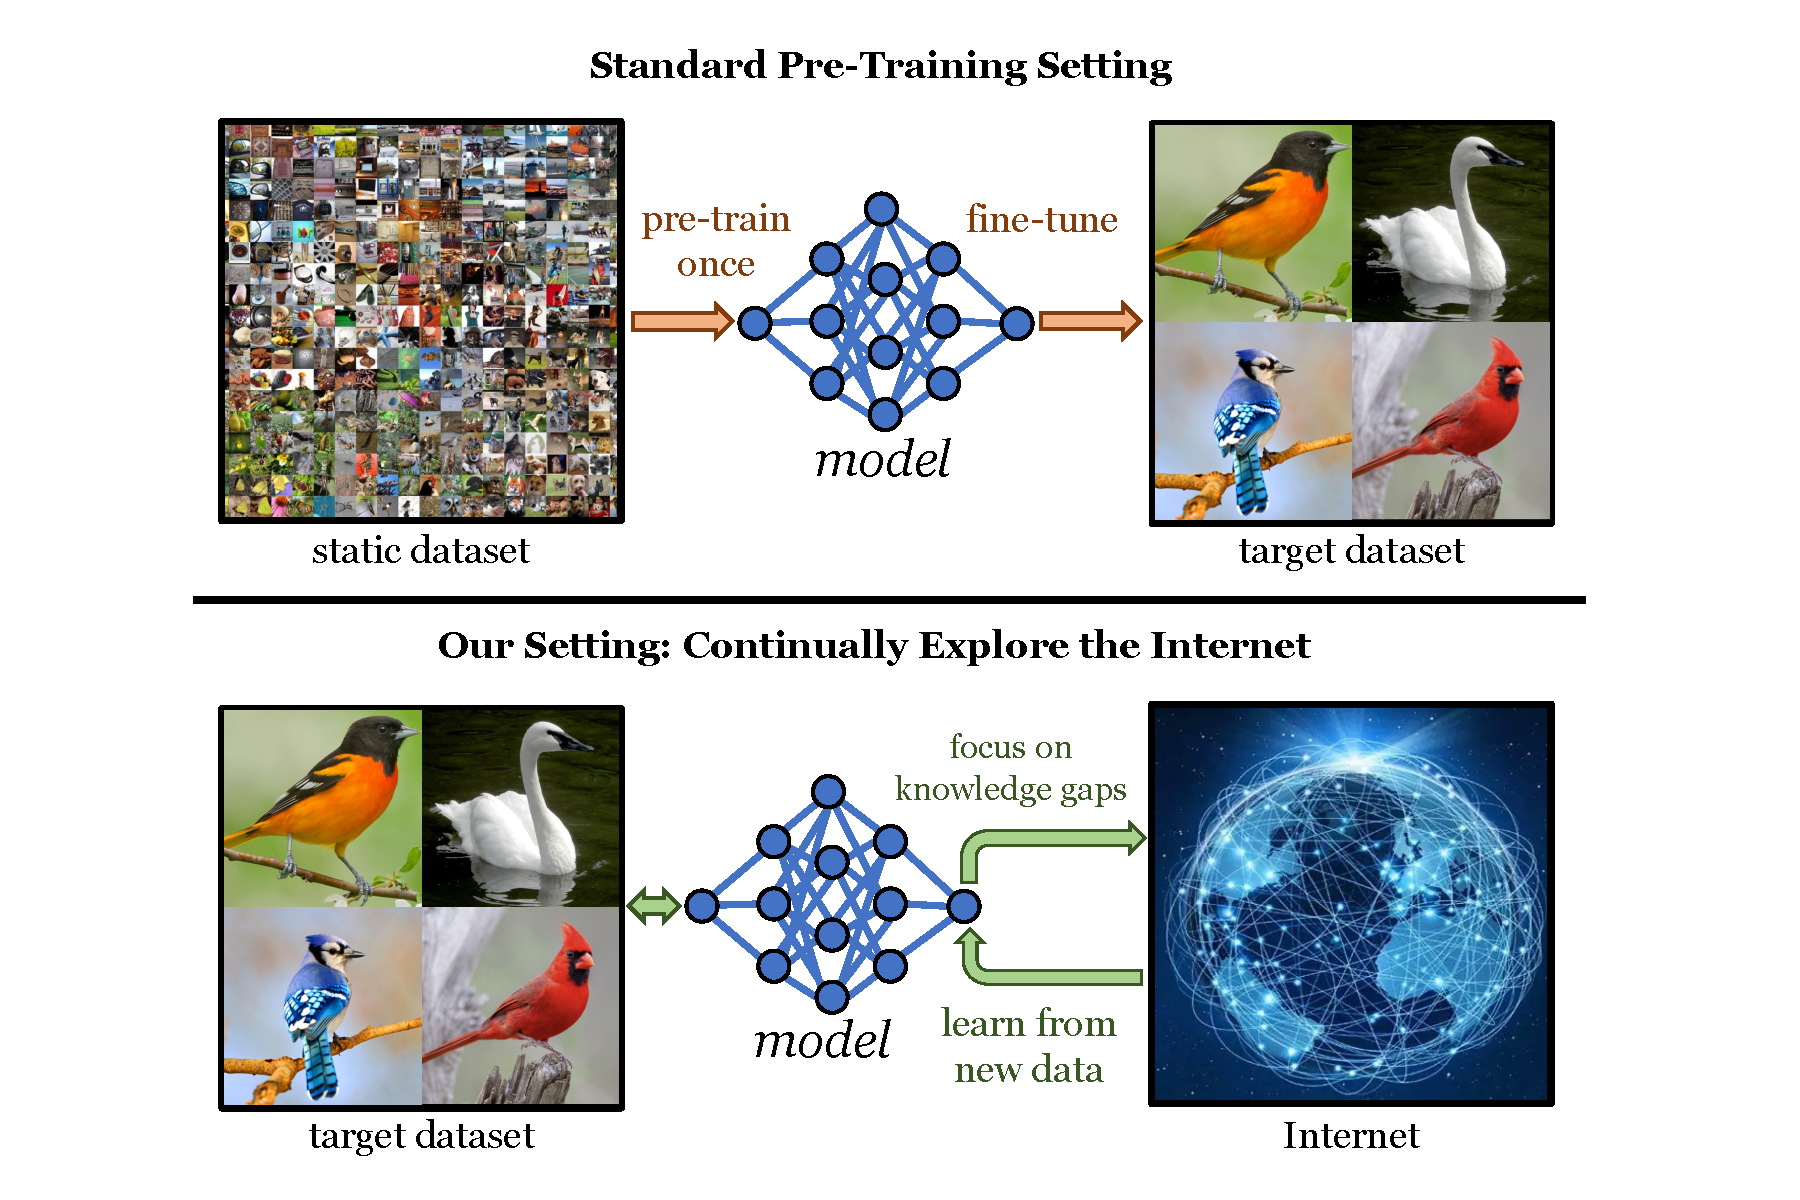
\includegraphics[width=0.8\linewidth]{figures/teaser2.pdf}
    % 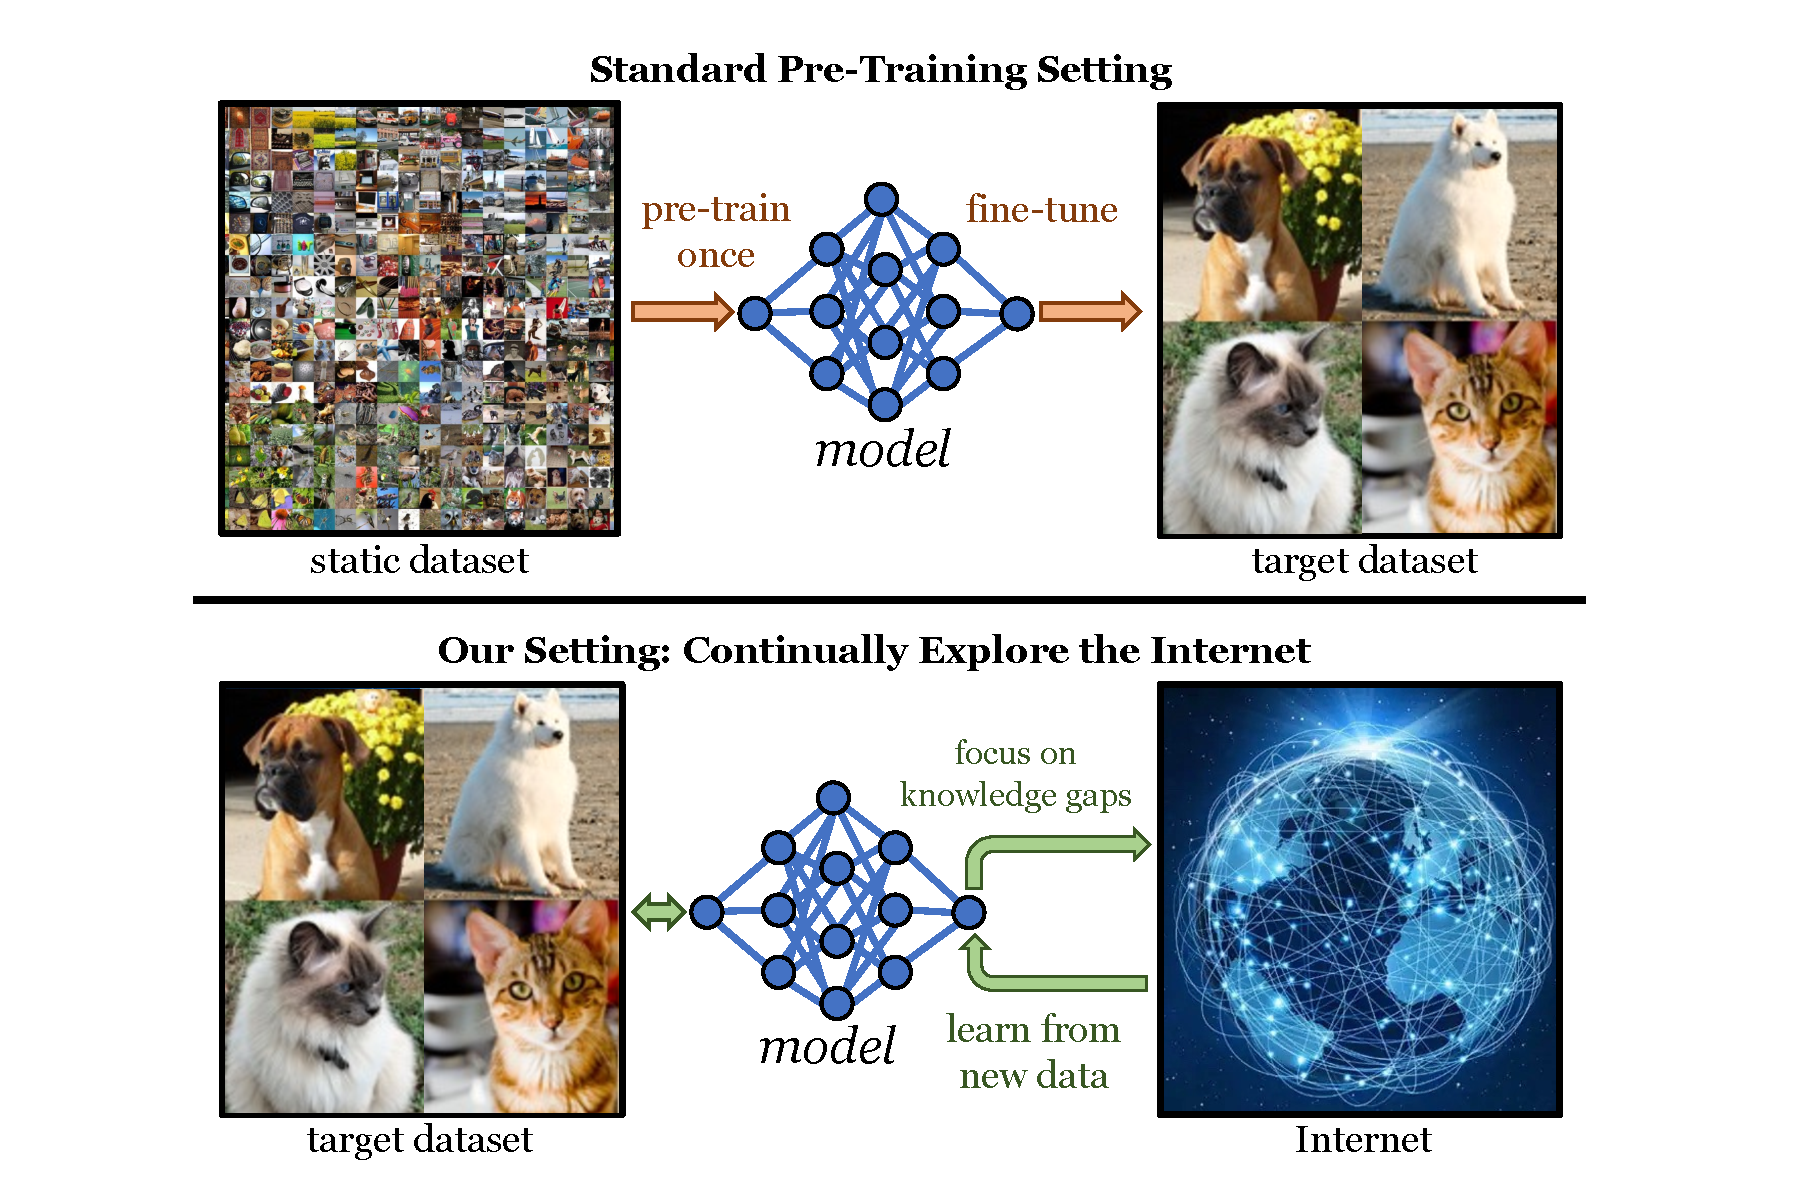
\includegraphics[width=\linewidth]{figures/alex.pdf}
    \caption{Given unlabeled data for a target task, our approach, Internet Explorer, searches the Internet to progressively find more and more relevant training data via self-supervised exploration.}
    \label{fig:teaser}
    % \vspace{-0.1in}
    \vspace{-0.15in}
\end{figure}

In this thesis, we rethink the idea of a \textit{\textbf{generic}} large-scale pretrained model and propose an alternate paradigm of training a rather small-scale but up-to-date model geared towards the \textit{\textbf{specific}} downstream task of interest. To train such a model, we go beyond static datasets and \textit{treat the Internet itself as a dynamic, open-ended dataset}. Unlike conventional datasets, which are expensive to increase and grow stale with time,
%are prone to bias, and yield suboptimal transfer performance when they contain little relevant data to the downstream task. 
the Internet is dynamic, rich, grows automatically, and is always up to date.
Its continuously evolving nature also means we cannot hope to ever download it or train a model, whether large or small, on all of it.
% But thinking pragmatically, do we even need to do so? Perhaps not.

We propose that the Internet can be treated as a special kind of dataset---one that exists out there, ready to be queried as needed to quickly train a customized model for a desired task.
% However, the issue is that the Internet is too big, and finding relevant images that help improve performance on a target dataset is a challenging endeavor.
We draw an analogy to reinforcement learning, where even though the task is known, finding a policy that can generate the desired behavior is non-trivial due to the high complexity of the state space. Hence, most approaches rely on some form of exploration to figure out what actions the agent should take so that it quickly finds high-reward states. Inspired by this analogy, we formulate a disembodied, online agent we call {\em Internet Explorer}, that actively searches the Internet using standard search engines to find relevant visual data that improve feature quality on a target dataset (see \cref{fig:teaser}). The agent's actions are text queries made to search engines, and the observations are the data obtained from the search.

The queries made by Internet Explorer improve over time. It cycles between searching for images on the Internet with text queries, self-supervised training on downloaded images, determining which images are relevant to the target dataset, and prioritizing what to search for next (see \cref{fig:method}). We also bootstrap Internet Explorer using existing pre-trained models such as MoCov3~\cite{he2020momentum} and obtain a significant boost on the target datasets.

Our setting is different from active learning~\cite{settles2009active}, where the goal is to selectively obtain labels for data points from a fixed dataset. In contrast, Internet Explorer continually expands the size of its dataset and requires no labels for training, even from the target dataset.
% However, we also show results in settings when the label set of the target dataset (not individual labels) are known.
Some prior works have also discussed ways to leverage the Internet as an additional source of data. NELL~\cite{carlson2010toward} proposed a way to continually scrape web pages to learn new concepts and relationships, which are periodically curated by a human in the loop. NEIL~\cite{chen2013neil} builds on the dictionary developed by NELL to search visual data to develop visual relationships. Both are semi-supervised methods to gather general ``common-sense'' knowledge from the Internet. In contrast, we perform an actively improving \textit{directed} search to perform well on target data, in a fully self-supervised manner. Recent work~\cite{jiang2021improving} follows a similar setting but searches a static dataset and not the Internet.

We evaluate Internet Explorer across 5 datasets, including 4 fine-grained datasets and PASCAL VOC.
% For simplicity, the search engine used is Google, but the method itself can work by searching on just image tags/captions as well.
We search for relevant images using Google; however, the method is compatible with any text-based search engine or even a static dataset (see \cref{subsec:search_engine_main}).
% \todo{prev sentence is out of date. mention laion / flickr}
We compare against several strong baselines, including CLIP, on downstream tasks. Note that CLIP acts as an oracle for our approach because it has likely already seen all or more queries that Internet Explorer makes.
In most scenarios, Internet Explorer either outperforms or matches CLIP oracle using only a single 3090 GPU desktop machine that runs for 30--40 hours, makes over 10K progressively improving queries, and downloads over 1M relevant Internet images for each target dataset.


\begin{figure}[t]
    \centering
    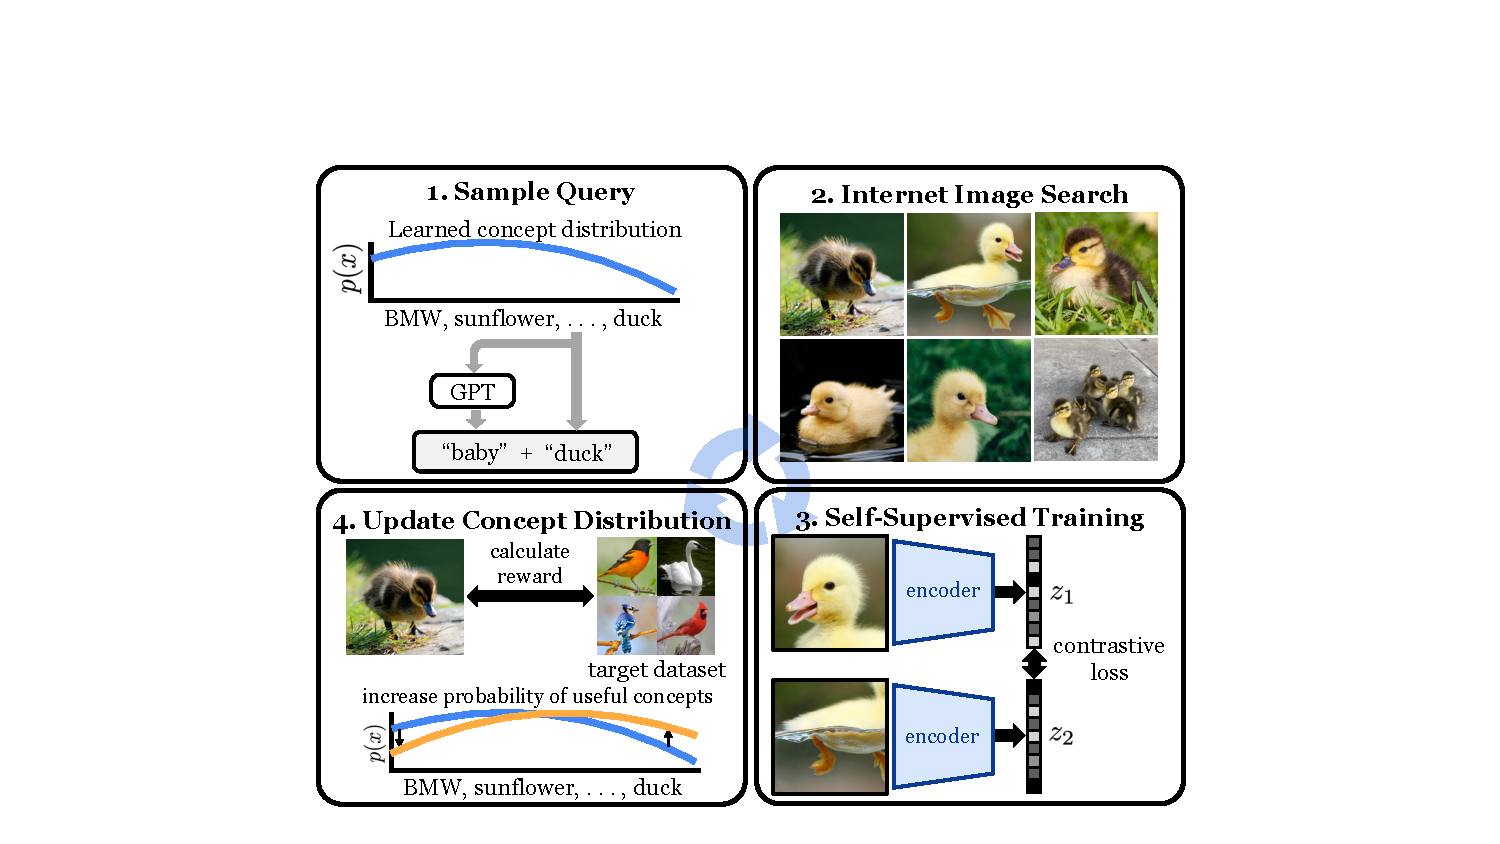
\includegraphics[width=0.85\linewidth]{figures/method_fig2.pdf}
    \caption{\textbf{Overview of Internet Explorer.} Our goal is to efficiently search the Internet for images that improve our performance on a target dataset.
        % In each iteration, we generate text queries by combining a concept sampled from a learned distribution with a GPT-generated descriptor. We query Google Images with the resulting phrase and download the top 100 image results. We add these images to the set of previously downloaded images and perform self-supervised learning on the combined dataset. 
        % Finally, we evaluate the relevance of the new images and increase the likelihood of the query and other related queries if the new images are similar to the target dataset.
        In each iteration, we first generate text queries by combining a concept sampled from a learned distribution with a GPT-generated descriptor (\S\ref{subsec:text_query_generation}, \ref{subsec:tiering}). Next, we query search engines with the resulting phrase and download the top 100 image results (\S\ref{subsec:text_to_image_search}, \ref{subsec:search_engine_main}). We add these images to the set of previously downloaded images and perform self-supervised training on the combined dataset (\S\ref{subsec:ssl}). Finally, we evaluate the relevance of the new images and update our concept distribution to increase the likelihood of similar queries if their images were similar to the target dataset (\S\ref{subsec:image_rel_reward},~\ref{subsec:unseen_reward}).
    }
    \label{fig:method}
    \vspace{-1em}
\end{figure}


%%% Local Variables:
%%% coding: utf-8
%%% mode: latex
%%% TeX-engine: xetex
%%% TeX-master: "../thesis"
%%% End:
\chapter{Method}
% This section provides a broad overview of foundational ideas
% and background material relevant to this thesis.
% In most chapters of this thesis, we include a deeper
% discussion of the related literature relevant to
% that material.




\section{Internet Explorer: An Online Agent}
% Ultimately, the goal of self-supervised learning is to learn a representation that is useful for a specific target dataset. 
% The most widely used application of machine learning is supervised learning with a known task and training dataset. 
% Practitioners typically try to improve model performance on a known target dataset by collecting additional labeled data or by fine-tuning a general-purpose pre-trained model. However, collecting data can be cumbersome and expensive, and general-purpose models may not be relevant enough to the task at hand. 
% We aim to improve performance for a known task by autonomously collecting more useful unlabeled data from the Internet. 
% With a known dataset,

We focus on the problem of efficiently improving representations for some target dataset by acquiring Internet data.
% improving performance on some prespecified task with a corresponding image dataset.
We make as few assumptions as possible and assume that we have only unlabeled training data from the target dataset. 
Successful representation learning in this setting would lead to better performance on the target dataset distribution for standard tasks like classification and detection, as well as others where the labels are not semantic (e.g., depth prediction or robotics).
% We can apply self-supervised methods directly to the target dataset, but performance quickly saturates, especially if the target dataset is small.
% We thus prioritize selectively collecting the data that is expected to improve the current model's performance on the target task. 
% Since we have a known target dataset, we can prioritize collecting data that is expected to be helpful for this task. We make as few assumptions as possible and assume that we have only unlabeled training data from the target domain, without any labels or information about what the dataset is about.
An overview of the Internet Explorer method is depicted in Figure~\ref{fig:method} and described in Algorithm~\ref{alg:internet_explorer}.
% }

\begin{figure}[!b]
    \centering
    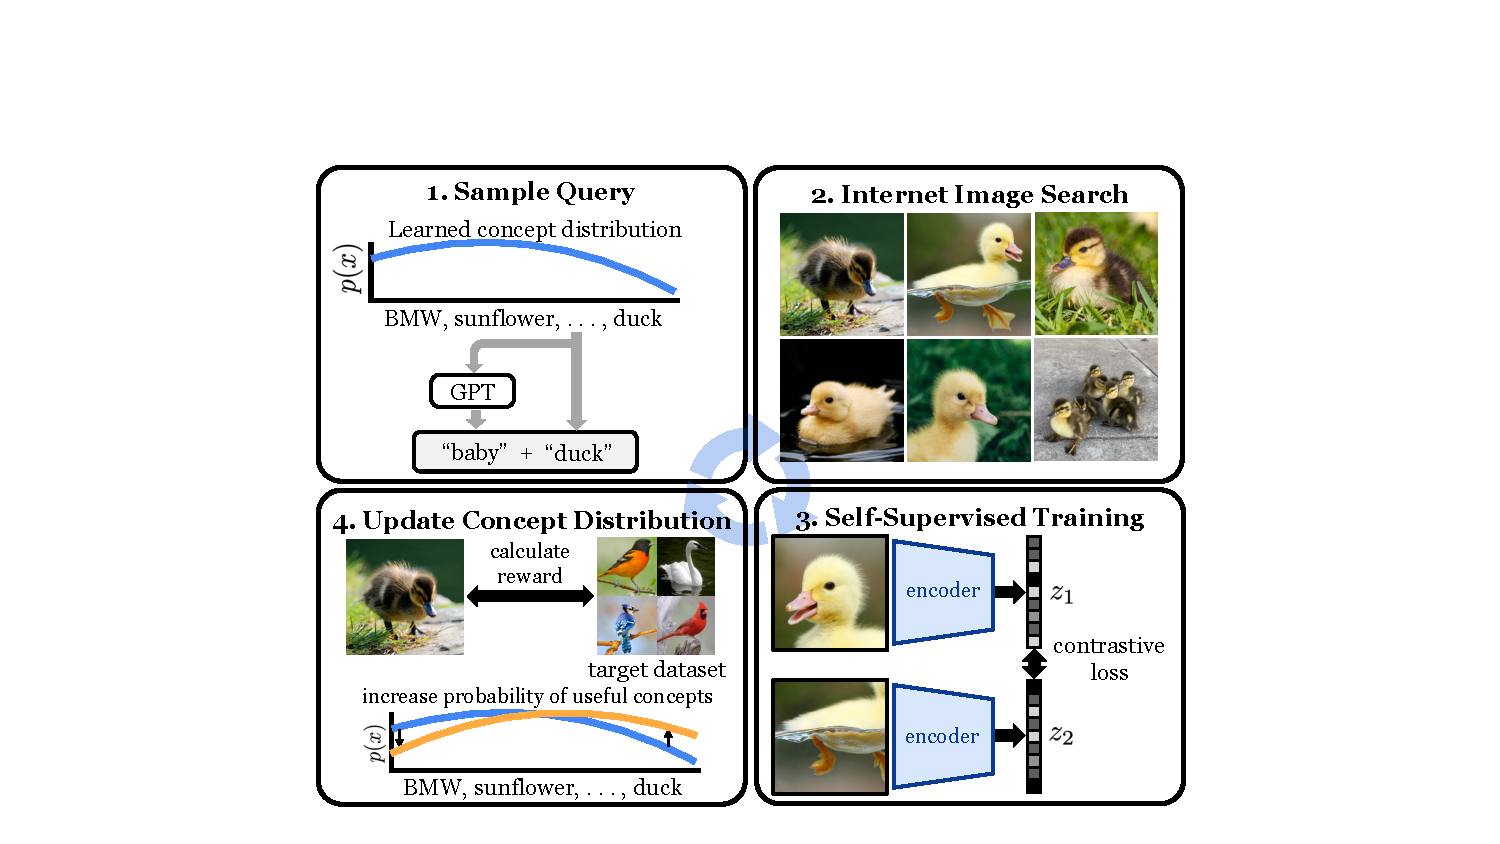
\includegraphics[width=0.8\linewidth]{figures/method_fig2.pdf}
    \caption{\textbf{Overview of Internet Explorer.} Our goal is to efficiently search the Internet for images that improve our performance on a target dataset.
        In each iteration, we first generate text queries by combining a concept sampled from a learned distribution with a GPT-generated descriptor (\S\ref{subsec:text_query_generation},~\ref{subsec:tiering}). Next, we query search engines with the resulting phrase and download the top 100 image results (\S\ref{subsec:text_to_image_search},~\ref{subsec:search_engine_main}). We add these images to the set of previously downloaded images and perform self-supervised training on the combined dataset (\S\ref{subsec:ssl}). Finally, we evaluate the relevance of the new images and update our concept distribution to increase the likelihood of similar queries if their images were similar to the target dataset (\S\ref{subsec:image_rel_reward},~\ref{subsec:unseen_reward}).
    }
    \label{fig:method}
\end{figure}

\subsection{Text-to-image Search}
\label{subsec:text_to_image_search}
% We would like a straightforward way to discover and download images from the full breadth of the Internet. 
% One directed approach to finding images online could be to progressively crawl the Web and prioritize which hyperlinks to expand based on some notion of ``usefulness''~\cite{kontogiannis2021tree}.
% However, this method has several major drawbacks. Ranking low-level hyperlinks (which of these web pages should I visit next) based on high-level semantic commands (I'd like to see pictures of Chihuahuas) is difficult to learn efficiently. Furthermore, each hyperlink expansion likely only yields a few new images, which almost certainly are not relevant to the concepts we care about. 
We discover and download images from the full breadth of the Internet by querying text-to-image search engines, which return images based on their captions and surrounding text. Text-to-image search is fast, returns diverse images from across the Internet, and enables searches for vastly different queries simultaneously. Note that text-to-image search is noisy and makes use of weak supervision (the image-text pairing on webpages). Thus, we only perform self-supervised training on the downloaded images. We use a public codebase to query Google Images, which can download the top 100 images for each query~\cite{hardikvasa, Joeclinton1}. We also try other search engines in \cref{subsec:search_engine_main}.
% We turn on SafeSearch, mark preference for photographs, and set the minimum image size to 350, the smallest setting available. 
% should we show an example of noisy results?

\subsection{Text Query Generation}
\label{subsec:text_query_generation}
% TODO: explain why a lot of thought goes into the query model. 
As text queries are our only input interface with the Internet, it is crucial that we can generate diverse queries that correspond to a variety of visual categories. Specificity is also important. Once a useful visual category is identified, generating fine-grained variants of the query is necessary to obtain data for all visual variations in the category.
% Language models could potentially be used to produce text queries, and reinforcement learning could be used to adjust their behavior based on the curiosity reward. Previous work found that RL worked well for preference-based training from human feedback~\cite{ziegler2019fine,stiennon2020learning,nakano2021webgpt}. However, we found that models such as BERT~\cite{devlin2018bert} or GPT-2~\cite{radford2019language} preferred generating human-centric phrases and did not generate sufficiently visually diverse queries, even with extensive prompt tuning. Thus, we avoid language models and 
We construct queries by combining two components: 
\begin{enumerate}[noitemsep,topsep=0pt]
    \item \textit{Concepts} specify semantic categories such as people, places, or objects. % Examples: golden retriever, daisy, BMW. 
    \item \textit{Descriptors} are modifiers that generate variations in appearance. % Examples: big, narrow, red. 
\end{enumerate}

We draw our concepts from the WordNet hierarchy~\cite{miller1995wordnet}, which consists of $146{,}347$ noun lemmas. Not all of these lemmas are visual, but the vocabulary still covers an incredible range of topics (see examples in \cref{sec:wordnet_lemmas}).
To generate a text query, we first sample a concept from a learned distribution over our vocabulary. This discrete distribution is defined by our estimates of how relevant each concept in the vocabulary is at the current time (see \cref{subsec:image_rel_reward} for details on estimating rewards and \cref{subsec:tiering} for the distribution).
Given a sampled concept, we can generate a descriptor by prompting a GPT-J language model~\cite{gpt-j} with examples of descriptor-concept pairs (details and examples in \cref{sec:gptj-descriptors}).
Finally, as shown in Step 1 of \cref{fig:method}, we simply concatenate the concept and descriptor. If our concept is ``duck'' and the GPT-generated descriptor is ``baby,'' our search engine query will be ``baby duck''.


\subsection{Self-supervised Training}
\label{subsec:ssl}
% EB NOTE:
% this section currently reads as: we use SSL, simsiam didnt work, but we use moco. moco details. we can also use other methods too
% IMO a potentially stronger stance: SSL is the core of our method, and it is compatible with any SSL algo and across many modalities. we choose images for X reason and moco for Y reason. then moco details

We use self-supervised learning (SSL) to learn useful representations from the unlabeled images that we download from the Internet. 
% We experimented with using SimSiam~\cite{chen2020exploring} as our base SSL algorithm due to its simplicity (no temperature, EMA rate, or loss weighting terms to tune), but found that it was unstable to train~\cite{li2022understanding}. 
Internet Explorer is compatible with any SSL algorithm that uses images or image-text pairs, including contrastive~\cite{he2020momentum,chen2020simple}, non-contrastive~\cite{grill2020bootstrap,zbontar2021barlow,bardes2021vicreg,caron2021emerging}, masking-based~\cite{bao2021beit,he2022masked}, or multimodal~\cite{radford2021learning} approaches. 
For speed and stability reasons, we use the MoCo-v3 algorithm~\cite{chen2021empirical}, which trains encoders $f_q$ and $f_k$ on augmentations $(x_1, x_2)$ of the same image to output vectors $q = f_q(x_1)$ and $k = f_k(x_2)$. $f_q$ is trained to minimize the InfoNCE loss~\cite{oord2018representation}:
\begin{align}
    \mathcal L_q = -\log \frac{\exp(q \cdot k^+ / \tau)}{\exp (q \cdot k^+ / \tau) + \sum_{k^-} \exp (q \cdot k^- / \tau) }
    \label{eq:moco_loss}
\end{align}
where $k^+$ corresponds to $f_k$'s output on the other augmentation of the image used to compute $q$, and the set of negative examples $\{k^-\}$ corresponds to $f_k$'s output on other images in the batch. The temperature $\tau$ is set to $1$ by default. $f_k$ consists of a base encoder, a projection MLP, and a prediction head, whereas $f_q$ is the exponential moving average of the base encoder and projection MLP from $f_k$. By training $q$ and $k^+$ to be similar across image augmentations, MoCo-v3 encourages the network to learn high-level semantic features. 

% In each iteration of our method, we use MoCo-v3 to fine-tune a ResNet-50 model~\cite{he2016deep} on a mixture of newly downloaded, previously downloaded, and target dataset images.
% Before turning to the Internet, we initialize our model using a MoCo-v3 checkpoint trained offline for 100 epochs on ImageNet and then
% another X steps on a mixture of ImageNet and the target dataset images. 
% fine-tuned with MoCo-v3 on the target dataset. Without using labels, we select the starting checkpoint for Internet Explorer by early-stopping on the SSL loss, which highly correlates with target accuracy~\cite{li2022understanding}.

Before turning to the Internet, we initialize a ResNet-50 model~\cite{he2016deep} using a MoCo-v3 checkpoint trained offline for 100 epochs on ImageNet and then fine-tuned on the target dataset. Without using labels, we select the best starting checkpoint by early stopping on the SSL loss, which highly correlates with target accuracy~\cite{li2022understanding}.
In each iteration of our method, we use MoCo-v3 to fine-tune on a mixture of newly downloaded, previously downloaded, and target dataset images.
% another X steps on a mixture of ImageNet and the target dataset images. 


% Even though we focus on using MoCo-v3, note that Internet Explorer is compatible with any SSL algorithm that uses images or image-text pairs, including contrastive~\cite{he2020momentum,chen2020simple}, non-contrastive~\cite{grill2020bootstrap,zbontar2021barlow,bardes2021vicreg,caron2021emerging}, masking-based~\cite{bao2021beit,he2022masked}, or multimodal~\cite{radford2021learning} approaches. 

\begin{algorithm}[t]
    \caption{$\texttt{Internet Explorer}$}
    \label{alg:internet_explorer}
\begin{algorithmic}[1]
    % \State {\bfseries Input:} target dataset $\mathcal D$, SSL algorithm $\mathbb{A}$, search engine $\texttt{SE}$, encoder $f: \mathbb{R}^{H \times W \times 3} \rightarrow \mathbb{R}^d$, image reward function $r$, vocabulary $\mathcal V = \{c_i\}_{i=1}^C$, $\#$ concepts/itr $M$, $\#$ query results/search $Q$, 
    % GPT-based concept $\rightarrow$ descriptor function $\texttt{GPTDesc}$, 
    % concept distribution function $\texttt{CalcProb}$
    \State {\bfseries Input:}
    \Statex \quad target dataset $\mathcal D$
    \Statex \quad SSL algorithm $\mathbb{A}$
    \Statex \quad search engine $\texttt{SE}$
    \Statex \quad encoder $f: \mathbb{R}^{H \times W \times 3} \rightarrow \mathbb{R}^d$
    \Statex \quad image reward function $r$
    \Statex \quad vocabulary $\mathcal V = \{c_i\}_{i=1}^C$, where $C$ is $\#$ concepts
    \Statex \quad $\#$ concepts/itr $M$
    \Statex \quad $\#$ query results/search $Q$
    \Statex \quad GPT-based concept $\rightarrow$ descriptor function $\texttt{GPTDesc}$
    \Statex \quad concept distribution function $\texttt{CalcProb}$
    \State Initialize replay buffer $\mathcal{B} \leftarrow \emptyset$
    \State Initialize concept distribution $p = \text{Uniform}\{1, C\}$
    \For{iteration $=1, 2, \dots$}
        \For{$i = 1, \dots, M$}
            \State Sample concept $c_i \sim p(\mathcal{V})$ \hfill (\S\ref{subsec:text_query_generation})
            \State Sample descriptor $d_i \gets \texttt{GPTDesc}(c_i)$ \hfill (\S\ref{sec:gptj-descriptors})
            \State Image search $\{I_j^i\}_{j=1}^Q  \leftarrow \texttt{SE}(d_i + c_i, Q)$ \hfill (\S\ref{subsec:text_to_image_search})
            % \State Calculate image rewards $r(f, \mathcal D, I_j^i)$
            % \State Calculate concept reward from image rewards
            % \State Calc.\ image rewards $\{r_{\text{img},j}^i\}_{j=1}^Q \gets r(f, \mathcal D, I_j^i)$
            % \State Calc.\ concept reward $r^i_{\text{concept}} \gets \frac 1 Q \sum_{j=1}^Q r_{\text{img},j}^i$
            \State Calc.\ reward $r_{c_i} \gets \frac 1 Q \sum_{j=1}^Q r(f, \mathcal D, I_j^i)$ \hfill (\S\ref{subsec:image_rel_reward})
        \EndFor
        \State $\mathcal B_{\text{new}} = \{I_j^1\}_{j=1}^Q \cup \dots \cup \{I_j^M\}_{j=1}^Q$
        \State SSL training: $\mathbb{A}(f, \mathcal D \cup \mathcal B \cup \mathcal B_{\text{new}})$ \hfill (\S\ref{subsec:ssl})
        \State Add to buffer: $\mathcal{B} \leftarrow \mathcal{B} \cup \texttt{Top50\%}(\mathcal B_{\text{new}}, r)$  % need to align r / r_concept to r_{c_i} above
        \State Predict all concept rewards $\mathbf{r}_{\text{concept}}$ from $\{r_{c_i}\}$ \hfill (\S\ref{subsec:unseen_reward})
        \State Update concept dist $p \leftarrow \texttt{CalcProb}(\mathbf{r}_{\text{concept}})$ \hfill (\S\ref{subsec:tiering})
    \EndFor
\end{algorithmic}
\end{algorithm}

\subsection{Image Relevance Reward}
\label{subsec:image_rel_reward}
We want to rank newly downloaded images by how much they improve our features for the target dataset. This allows us to (a) prioritize taking gradient steps on useful images, and (b) understand what to search for in subsequent iterations. Unfortunately, it is challenging to directly measure the effect of an individual training example on performance. Numerous techniques have been proposed~\cite{koh2017understanding,feldman2020neural,paul2021deep,ilyas2022datamodels}, but they all require extensive and repeated training on new images to estimate their impact. 

% Instead of trying to precisely measure what is learned from each image, we rank the images by their distance in representation space to the target dataset images. The images most similar to the target dataset induce larger contrastive loss, since each $\exp(q \cdot k^-)$ term in the denominator of Eq.~\ref{eq:moco_loss} is larger when the negative examples $\{k^-\}$ are closer to $q$.
Instead of trying to precisely measure what is learned from each image, we use its similarity to the target dataset as a proxy for being relevant to training.
We rank the downloaded images by their similarity in representation space to the target dataset images; those most similar to the target dataset induce larger contrastive loss since each $\exp(q \cdot k^-)$ term in the denominator of Eq.~\ref{eq:moco_loss} is larger when the negative examples $\{k^-\}$ are closer to $q$.
These ``hard negatives''~\cite{robinson2020contrastive,schroff2015facenet,oh2016deep,harwood2017smart,wu2017sampling,ge2018deep} yield larger and more informative gradients and should result in the biggest improvement in representation quality.
% The best way to improve performance on the target dataset is by finding data that \textit{looks like the target dataset.} Figure~\ref{fig:in_vs_flowers} shows that self-supervised learning on just 2040 Flowers102 images outperforms self-supervised pre-training on ImageNet, which contains 1.2 million images ($628\times$ as much data). Pre-training on only flower images only requires about 2\% the training time as ImageNet pre-training.
% Motivated by this, 
% We heuristically want to find Internet images similar to the ones in the target dataset, in hopes that they most efficiently improve self-supervised training. Thus, we formulate a curiosity reward (higher is better) to prefer images that are most similar in representation space to the target dataset images.
% We want to find the best Internet images for future self-supervised training. 
% As shown in Figure~\ref{fig:curiosity_reward}, the curiosity reward for a particular image is its representation's negative distance to its closest neighbor in the target dataset.
Thus, overloading notation for $k$, we compute the reward for a particular image as its representation's average cosine similarity to its $k$ closest neighbors in the target dataset. Given an image encoder $f_k: \mathbb{R}^{H\times W\times 3} \rightarrow \mathbb{R}^d$, an unlabeled target dataset $\mathcal D = \{ x_i \}_{i=1}^N$, and a new image $y$ to evaluate, the reward is calculated:
\begin{align}
    r(f_k, \mathcal D, y) =
        \max_{\substack{I \subset \{1, \ldots, N\}; \\ |I| = k}}
        \frac{1}{k} \sum_{i \in I} S_{\cos}\left(f_k(x_i), f_k(y)\right)
\end{align}
where $S_{\cos}$ is the cosine similarity. A previous metric for identifying relevant data~\cite{jiang2021improving} used $k=1$ nearest neighbors, 
% but we found that this was too noisy and enabled high rewards for images unrelated to almost all of the target dataset. 
but we found that this was too noisy and allowed high rewards for outlier target images to distract our search.
We instead use $k=15$ to improve the accuracy of our relevance estimation.
In \cref{subsec:reward_analysis}, we compare our reward to alternatives and explore their failure modes. This reward is used for two purposes: determining which of the downloaded images to train on and, subsequently, which concepts would be useful to search for next.

\vspace{-0.06in}
\paragraph{Which images to train on.}
Many newly downloaded images are not worth training on, since they come from unrelated queries or are noisy results from the search engine.
Thus, at the end of each iteration, we rank the newly downloaded images by their reward and save the top $50\%$ to a replay buffer that we maintain across iterations. In subsequent iterations, we continue training on this filtered data.

\vspace{-0.06in}
\paragraph{Determining which concepts are useful.}
When we search for a concept and get back $Q$ image results $\{ I_i \}_{i=1}^Q$, we take the average of the top 10 image-level rewards $r_i = r(f_k, \mathcal D, I_i)$ and use that as a \textit{concept-level score}. This gives us an accurate measure of the relevance of a particular query and reduces the impact of noisy search results. 



\subsection{Estimating Reward for Unseen Concepts}
\label{subsec:unseen_reward}

\subsubsection{Concept Embeddings}
Since our vocabulary contains hundreds of thousands of concepts, it would be inefficient to test whether \emph{each} possible query yields relevant images. Luckily, we can estimate the quality of queries by using the observed rewards of the queries searched so far. Humans can do this effortlessly due to our understanding of what each concept means. To us, it is obvious that if querying ``duck'' yielded useful images for this dataset and ``BMW'' did not, then we should search for more images of animals and not cars. We want to give our method the same understanding of concept meaning, so we embed our $146{,}347$ WordNet concepts into a 384-dimensional space using a pre-trained sentence similarity model~\cite{reimers2019sentence}. We provide relevant context about each concept to the text embedding model by using additional information from WordNet in the following template:

\begin{quote}
    {\tt {\small \{lemma\} (\{hypernym\}): \{definition\}}}
\end{quote}
For example, the text that is embedded for the concept ``Chihuahua'' is:

\begin{quote}
    {\tt {\small Chihuahua (toy dog): an old breed of tiny short-haired dog with protruding eyes from Mexico held to antedate Aztec civilization.}}
\end{quote}


\subsubsection{Predicting Rewards}
Now that we have a representation of each concept, we can estimate the reward for untried concepts by using the rewards of concepts that we have already searched for.
We use Gaussian process regression (GPR)~\cite{williams1995gaussian} over the text embeddings $\{\mathbf{e}_i\}$ to predict the concept-level reward $r(\mathbf{e}_i)$ for untried concepts. 
GPR models the function outputs for any set of inputs $\{r(\mathbf{e}_i)\}$ as jointly Gaussian random variables. 
The covariance of any two variables $r(\mathbf{e}_i)$ and $r(\mathbf{e}_j)$ is determined by the kernel $k(\mathbf{e}_i, \mathbf{e}_j)$, which we set as the default RBF kernel $k(\mathbf{e}_i, \mathbf{e}_j) = \exp(\frac{-\|\mathbf{e}_i - \mathbf{e}_j\|_2}{2})$. 
Given the observed rewards for concepts $R_{obs} = \{r(\mathbf e_i)\}$, GPR calculates the posterior distribution over the rewards for an unobserved concept $\mathbf e'$, $P(r(\mathbf e') \mid \{r(\mathbf{e}_i)\} = R_{obs})$. Given that the joint distribution  $P(\{r(\mathbf{e}_i)\}, r(\mathbf{e}'))$ is Gaussian, the posterior is also Gaussian with mean $\mu(\mathbf e')$ and variance $\sigma{(\mathbf e')}^2$. The locality provided by the RBF kernel enables reasonable reward predictions, and having a distribution over rewards instead of a point estimate allows us to explore potentially good concepts. We encourage exploration by setting the score of unobserved concepts to $\mu(\mathbf{e}_i) + \sigma(\mathbf{e}_i)$.

% a practical issue: GPR slows down a ton as the number of points increases. for this reason, after 10 iterations (256 queries * 100 images * 10 iters = 256k points), we switch to a simple ridge regression model. this is a good tradeoff because we have a lot of data by this point, and we don't need to explore as much anymore.

A practical issue is that GPR does not scale well to large numbers of points, and fitting the model after each iteration becomes prohibitively slow. To address this, we use GPR for the first 10 iterations ($256$ queries $\times$ $100$ images $\times$ $10$ iterations $\approx 256{,}000$ points), and then switch to a simple ridge regression model that predicts solely the mean rewards $\mu(\mathbf{e}_i)$---and thus we eliminate the exploration term $\sigma(\mathbf{e}_i)$ from the reward prediction. This is a good tradeoff because we have a lot of data by this point, and we don't need to explore as much anymore.
The number of iterations at which we switch to ridge regression is a hyperparameter that can be tuned to balance exploration and exploitation + speed. We found that 10 iterations to work well in practice.


\subsection{Query sampling distribution}
\label{subsec:tiering}

\begin{figure}[t]
    \centering
    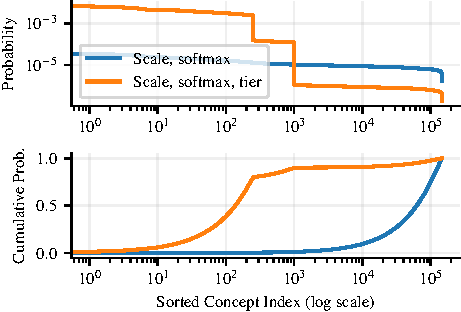
\includegraphics[width=0.7\linewidth]{figures/sampling_dist_shorter.pdf}
    \caption{\textbf{Learned concept sampling distribution.} Given estimated scores for each of the $146{,}347$ concepts, we need to choose how often to sample each one in order to balance exploration and exploitation.
    \textbf{Top:} we scale our scores to a desired temperature, then take the softmax to obtain a distribution over concepts. Finally, we create tiers so that the top 250 concepts have $80\%$ of the probability mass, and the next 750 have $10\%$. This ensures that we sample enough from the top $1{,}000$ concepts while still exploring other concepts with lower scores.
    \textbf{Bottom:} the top 1000 concepts are only sampled a tiny fraction of the time without tiering.}
    \label{fig:sampling_dist}
    \vspace{-0.12in}
\end{figure}

Once we have estimates for the quality of each concept, how do we determine what to search for next?
% We have two desiderata: 
    % \begin{enumerate}
%     \item Sufficient exploration of potentially good queries. 
%     % \item Sample the top concepts frequently enough, so that we get enough relevant training data for SSL. 
%     \item Frequent enough sampling of the top concepts, so that we get good relevant training data for SSL. 
% \end{enumerate}
We face the age-old dilemma of exploration versus exploitation:
% \begin{enumerate}[noitemsep,topsep=0pt]
%     \item We need to sample the top concepts frequently enough to get relevant training data for SSL.
%     \item At the same time, we need sufficient exploration of promising untried concepts.
% \end{enumerate}
we need to sample the top concepts frequently enough to get relevant training data for SSL, while at the same time, we need sufficient exploration of promising untried concepts.
% A greedy approach, like only searching for the top $C$ concepts with the highest estimated reward, results in poor exploration of untried concepts. Instead, w

We use a sampling-based approach based on Boltzmann exploration~\cite{sutton1991dyna}. Boltzmann exploration samples based on a scaled softmax distribution $ p(c_i) \propto \exp(r(c_i)/\tau)$, where  
% maybe make reference to bandits, ucb, bayesian optimization, soft q learning 
% \begin{align}
%     p(c_i)  = \frac{\exp(r(c_i)/\tau)}{\sum_j \exp(r(c_j)/\tau)}
% \end{align}
$\tau$ is the temperature scaling.
However, with a large vocabulary (action space) of $146{,}347$ concepts, it becomes difficult to tune $\tau$ so that we sample the top concepts frequently enough without being too skewed. 
Thus, we define a ``tiering function'' to adjust the probability mass in specified intervals of our distribution. Given a sorted discrete probability distribution $p$, interval boundaries $T_0 =0 < T_1 < \dots < T_n$, and interval masses $\Delta_0, \dots, \Delta_{n-1}$ such that $\sum_i \Delta_i = 1$,  tiering computes a new distribution: 
\begin{align}
    p_i^{\text{tier}} = \Delta_j \frac{p_i}{\sum_{k=T_j}^{T_{j+1}} p_k} \;\;\; \text{for } j \text{  s.t.  }T_j \leq i < T_{j+1} 
\end{align}
$p^{\text{tier}}$ is a new distribution such that $\sum_{k=T_j}^{T_{j+1}} p^{\text{tier}} = \Delta_j$. We use $T_0=0$, $T_1=250$, $T_2=1{,}000$, $T_3=146{,}347$, $\Delta_0=0.8$, $\Delta_1 = 0.1$, and $\Delta_2=0.1$.
Simply put: we give the highest-ranked $250$ concepts $80\%$ of the probability mass, the next $750$ concepts $10\%$, and all remaining concepts $10\%$.
Figure~\ref{fig:sampling_dist} shows that tiering the scaled softmax distribution samples frequently enough from the top concepts while a vanilla scaled softmax distribution does not.
Note that the untiered distribution would sample the top $1000$ concepts only $\approx 0.1\%$ of the time, while the tiered distribution samples them $90\%$ of the time.

% Things to mention 
% \begin{itemize}
%     \item comparison of different ways of computing the text embeddings. describe just embedding the concepts, vs embedding the concept and the wikipedia summary
%     \item histograms of the text embedding similarity
%     \item ways of purifying the similarity matrix
%     \item TODO: think about rewarding quality over quantity
% \end{itemize}

\subsection{Provable speedup in relevant query identification}
\label{subsec:provable_speedup}
We now show that our method can provably speed up the time to identify all relevant concepts in a dataset.
Assume that our vocabulary of $n$ concepts contains $c \cdot s \ll n $ relevant concepts, which are partitioned into $c$ disjoint clusters of size $s$. We want to discover every relevant concept by sampling concepts uniformly at random (with replacement) to test. Assume that sampling a concept conclusively tells us whether it is relevant. Furthermore, assume that we could optionally use a Gaussian process regression model which, if we've sampled a relevant concept, tells us that all the concepts in its cluster are also relevant.\\

\begin{restatable}{lemma}{lemmaspeedup}
    \label{lemma:speedup}
    Let $T_{base}$ be the expected time to identify every relevant concept without the GPR, and $T_{GPR}$ be the expected time when exploiting the additional knowledge from the GPR. Then, $T_{base} = n H_{c \cdot s}$, $T_{GPR} = \frac{nH_{c}}{s}$, and the speedup from GPR is $\frac{T_{base}}{T_{GPR}} \approx s \log s$.
\end{restatable}

\begin{proof}
    This problem is a variant of the coupon collector problem. Let's first compute $T_{base}$ as the sum of expected times $t_i$ to identify the next relevant concept. 
    \begin{align}
        T_{base} &= \sum_{i=1}^{cs} t_i \\
                 &= \sum_{i=1}^{cs} \frac{1}{p_i} \\
                 &= \sum_{i=1}^{cs} \frac{n}{cs + 1 - i} \\
                 &= n \sum_{i=1}^{cs} \frac{1}{cs + 1 - i} \\
                 &= n H_{cs}
    \end{align}
    where $H_{cs}$ is the $cs$th harmonic number. Similarly, we can compute $T_{GPR}$ as the sum of expected times $t_i$ to identify the next relevant cluster.  
    \begin{align}
        T_{GPR} &= \sum_{i=1}^{c} t_i \\
                 &= \sum_{i=1}^{c} \frac{1}{p_i} \\
                 &= \sum_{i=1}^{c} \frac{n}{s (c + 1 - i)} \\
                 &= \frac{n}{s} \sum_{i=1}^{c} \frac{1}{c + 1 - i} \\
                 &= \frac{nH_{c}}{s}
    \end{align}
    The speedup is then $\displaystyle \frac{T_{base}}{T_{GPR}} = s \frac{H_{cs}}{H_c} \approx s \log s$.
\end{proof}

We find that in practical settings (e.g., the Pets example analyzed in Fig.~\ref{fig:reward_over_training}), we can accurately predict how many samples are required to discover all useful concepts. If the vocabulary size is $n \approx 150{,}000$, the number of clusters is about $c = 2$ (one for cats and one for dogs), and the size of each cluster is about $150$, then $T_{GPR} = 1500$, which roughly matches the $9 \times 256 = 1792$ queries it took to discover both cats and dogs in the Pets dataset.


\section{Method Details}

% We draw our concepts from the WordNet hierarchy~\cite{miller1995wordnet}, which consists of $146{,}347$ noun lemmas. Not all of these lemmas are visual, but the vocabulary still covers an incredible range of topics.
% % For reference, here are 6 randomly sampled concepts:  {\tt {\small `sleep talking', 
% % `beach wagon', `Balearic Islands', `borosilicate', `genus Loranthus', `humpback whale'}}.
% We can generate descriptors for each concept by prompting a GPT-J language model~\cite{gpt-j} with examples of descriptor-concept pairs (details in the supplementary).
% % For reference, here are 7 randomly sampled descriptors for ``labrador retriever'': {\tt {\small `friendly', `short', `long-legged', `big', `fast', `blue-eyed', `handsome'}}.

\subsection{WordNet Lemmas}
\label{sec:wordnet_lemmas}
We draw our concepts from the WordNet hierarchy~\cite{miller1995wordnet}, which consists of $146{,}347$ noun lemmas. For reference, here are 32 randomly sampled concepts:
\begin{quote}
{\tt { 
% `sleep talking', `beach wagon', `Balearic Islands', `borosilicate', `genus Loranthus', `humpback whale'
"resolution",
"lodgment",
"phycobilin",
"acidosis",
"widening",
"human face",
"family Crassulaceae",
"sail",
"Ipomoea imperialis",
"Davis",
"prothrombin",
"cease",
"marsh clematis",
"major power",
"chump change",
"madcap",
"junky",
"pere david's deer",
"make-up",
"genus Rumex",
"gape",
"Brachychiton populneus",
"bell morel",
"wain",
"friendly",
"Principe",
"bottle green",
"glycerol trimargarate",
"water-shield",
"San Joaquin River",
"woodsman",
"pin".
}}
\end{quote}

\subsection{GPT-J Descriptor Prompting}
\label{sec:gptj-descriptors}
We use GPT-J-6B~\cite{gpt-j}, a free, open-source autoregressive language model, to generate useful descriptors for a given concept. We use the following prompt template: 
\begin{itemize}
    \item[] \texttt{"What are some words that describe the quality of `\{concept\}'?} 
    \item[] \texttt{The \{concept\} is frail.}
    \item[] \texttt{The \{concept\} is red.}
    \item[] \texttt{The \{concept\} is humongous.}
    \item[] \texttt{The \{concept\} is tall.}
    \item[] \texttt{The \{concept\} is"}
\end{itemize}

We sample completions with a temperature of 0.9 and a max length of 100 tokens. We truncate the completion after the first comma, period, underscore, or newline character (including the special character). If the truncated completion is degenerate and contains a duplicate of the concept, we resample another completion. After successfully sampling a descriptor, we prepend it to the concept and use the resulting phrase as our search query. 

% - TODO: put in a page of examples.   
% - Pencil: 'fragile', 'huge!', 'too big', 'colorful', 'dark', 'too soft', 'blunt', 'narrow', 'round', 
% 'blue', 'black', 'a soft piece of wood', 'thick', 'heavy', 'light', 'short'
% - TODO: These descriptors generally 
% - Our prompt can be easily 

For reference, here are 32 randomly sampled descriptors for ``labrador retriever'':
% {\tt {\small `friendly', `short', `long-legged', `big', `fast', `blue-eyed', `handsome'}}.
\begin{quote}
{\tt { 
% `sleep talking', `beach wagon', `Balearic Islands', `borosilicate', `genus Loranthus', `humpback whale'
"a good-looking dog",
"very gentle",
"a",
"brown",
"lovable",
"a strong runner",
"a male or a female",
"sturdy",
"agile",
"a strong",
"beautiful",
"a male",
"kind",
"long-haired",
"a male or a female",
"a good-looking dog",
"gentle",
"medium",
"loyal",
"very gentle",
"blue-eyed",
"sturdy",
"blue-eyed",
"a retriever",
"kind",
"loyal",
"large",
"brown",
"good-natured",
"gentle",
"large",
"small".
}}
\end{quote}



\subsection{Concept Vocabulary Size}
\label{sec:concept_vocab_size}
As stated in \cref{subsec:text_query_generation}, our vocabulary comprises the $146{,}347$ noun lemmas in the WordNet hierarchy. Thus, in all our experiments, Internet Explorer only searches for WordNet terms (plus the class names, if we have knowledge of the label set). We found that this worked quite well for these standard benchmarks. Note that expanding the vocabulary (e.g., adding technical terms relevant to a specific topic) can easily be done by adding those terms to the list of possible concepts. One easy extension would be to add page titles and frequent unigrams and bigrams from Wikipedia, as was done to generate the CLIP training set~\cite{radford2021learning}. Doing so would expand our vocabulary to roughly $500{,}000$ total concepts. 

\subsection{Query Model Details}
\label{sec:query_model_details}
\paragraph{Temperature for concept distribution}
After estimating scores $r(c_i)$ for each concept $c_i$, we do a temperature-scaled softmax, followed by the tiering operation described in \cref{subsec:tiering}. We compute the temperature $\tau$ such that 
\begin{align}
     \text{SMR} = \frac{\max_i r(c_i) - \min_i r(c_i)}{\tau}
\end{align}
where the ``softmax range'' $\text{SMR} \in \mathbb R$ is the desired gap between the largest and smallest scores after temperature scaling. After the softmax $p(c_i) \propto \exp(r(c_i) / \tau)$, the softmax range determines the likelihood ratio of most likely concept to least likely concept: 
\begin{align}
    \frac{\max_i p(c_i)}{\min_i p(c_i)} &= \frac{\max_i \exp(r(c_i) / \tau)}{\min_i \exp(r(c_i) / \tau)} \\
      &= \exp \left(\frac{\max_i r(c_i) - \min_i r(c_i)}{\tau}\right) \\
    &= \exp(\text{SMR})
\end{align}
Thus, SMR is an easy way to specify the relative likelihood of the highest and lowest scoring concepts and achieve a desired exploration-exploitation balance. 


\paragraph{Label set-guided vocabulary}
To reduce our search space in the label set-guided setting, in which we know the English names of the classes a priori, we generate a subset of the WordNet vocabulary that contains only the top-$10\%$ most semantically-relevant concepts to each target dataset.
We use a pre-trained text embedding model~\cite{reimers2019sentence} to generate $384$-dimensional embeddings for each concept in WordNet, using the same template described in \cref{subsec:unseen_reward}

\begin{quote}
{\tt {\small \{lemma\} (\{hypernym\}): \{definition\}}}.
\end{quote}

To generate a similar embedding for concepts in target datasets, we use the summary from Wikipedia in place of the definition and the ``category'' of the target dataset (shown in \cref{tab:dataset_categories}) in place of the hypernym:

\begin{quote}
{\tt {\small \{label\} (\{category\}): \{summary\}}}.
\end{quote}


\begin{table}
    \centering
    \begin{tabular}{ll}
    \toprule
        Dataset & Category \\
    \midrule
        Oxford Flowers102 & Flower \\
        Oxford IIIT Pets & Pet \\
        Food101 & Food \\
        Birdsnap & Bird \\
        VOC2007 & Object \\
    \bottomrule
    \end{tabular}
    \caption{\textbf{Target Dataset ``Category''}.
    }
    \label{tab:dataset_categories}
\end{table}

After generating the embeddings for each concept in the target dataset, we find the $k$-NN distance for each WordNet concept to the target dataset embeddings, where $k$ is chosen to be $1/3$ the size of the class label set.
We then rank the concepts in WordNet by the distance and take the closest $10\%$ of terms as our subset. This subset is used for all methods in the label set-guided setting, including the random exploration methods. 






\subsection{Training Details}
In each iteration, we download roughly 25k candidate images, since we download up to 100 images for each of the 256 queries. Given this set $\mathcal C$ of candidate images, we sample $\text{PCR} \times |\mathcal C|$ images from the union of the replay buffer $\mathcal B$ and the target dataset training images $\mathcal D$. PCR (past data to candidate data ratio) is a scalar value that determines how much old data vs new data to train on at every iteration. We set $\text{PCR}=2$ for all experiments. We perform $10$ epochs of training over the union of the new candidate data and the sampled replay buffer and target dataset images. 

\subsection{Hyperparameters}
% privilege ratio, privilege gamma 
% k 
% GP 

\cref{tab:hyperparameters} shows our hyperparameter values, which are shared across datasets. We perform minimal hyperparameter tuning and copy most of the values from the MoCo-v3~\cite{chen2021empirical} ResNet-50 configuration. 
We will also release our code upon acceptance, which we hope will clarify any remaining implementation details and make it easy for the community to reproduce and build on our work. 
\begin{table}
    \centering
    % \begin{adjustbox}{width=\linewidth}
    \begin{tabular}{ll}
    \toprule
        Hyperparameter & Value \\
    \midrule
        Architecture & Resnet-50~\cite{he2016deep} \\
        Optimizer & LARS~\cite{you2017large} \\
        Batch size & $224$ \\
        Learning rate & $0.8 \times \frac{224}{256}$ \\
        Learning rate schedule & constant \\
        MoCo momentum & $0.9985$ \\
        RandomResizedCrop min crop area & $0.2$ \\
        % PCR & 2? \\
        Queries per iteration & $256$ \\
        Requested images per query & $100$ \\
        Min images per query & $10$ \\    
        Softmax range (SMR) & $3$ \\
        PCR & $2$ \\
        Epochs per iteration & $10$ \\
    \bottomrule
    \end{tabular}
    % \end{adjustbox}
    \caption{\textbf{Internet Explorer hyperparameters}.}
    \label{tab:hyperparameters}
\end{table}


\subsection{Image Licenses}
Internet Explorer uses images that were indexed by a web crawler (Google Images and LAION) or uploaded to Flickr. The images and their rights belong to their respective owners; we use, download, and train on them under fair use guidelines for research. 

%%% Local Variables:
%%% coding: utf-8
%%% mode: latex
%%% TeX-engine: xetex
%%% TeX-master: "../thesis"
%%% End:

\chapter{Experimental Setting and Results}
% This section provides an overview of the experimental setting used to evaluate Internet Explorer, as well as the key results of our experiments in these settings.
This section provides an overview of the experimental setting used to evaluate Internet Explorer, as well as detailed results and analysis of our experiments in these settings.

\section{Experimental Setting}
\subsection{Self-supervised Exploration}
% explain why this setting is important, and explain the baselines 
To make Internet Explorer as widely applicable as possible, we first evaluate it in a setting where we assume no prior knowledge of the contents of the images 




We assume that we have an unlabeled target dataset of images for which we would like to learn useful visual features. We compare three methods:
% EB: we should consider a better abbreviated method name. how about: IE, IE+?
% \begin{enumerate}[noitemsep,topsep=0pt]
%     \item Random: sample queries uniformly at random from the vocabulary. 
%     \item Ours: sample queries from our learned concept distribution. 
%     \item Ours++: additionally use GPT-generated descriptors
% \end{enumerate}
% \begin{enumerate}[noitemsep,topsep=0pt]
\begin{enumerate}
    \item Random: sample concepts uniformly from the vocab. 
    \item Ours: sample concepts from our learned distribution. 
    \item Ours++: additionally use GPT-generated descriptors.
\end{enumerate}
% lack of label knowlege makes this challenging but also generally applicable
% This setting is challenging because we have to explore to discover what concepts are useful for our target dataset, without any prior knowledge of what those concepts might be. 
The lack of label knowledge makes this setting challenging, but also very general. Our method is forced to explore the space of concepts to discover what is useful for the target dataset, without any prior knowledge of what might be useful.

\begin{figure*}[t]
    \centering
    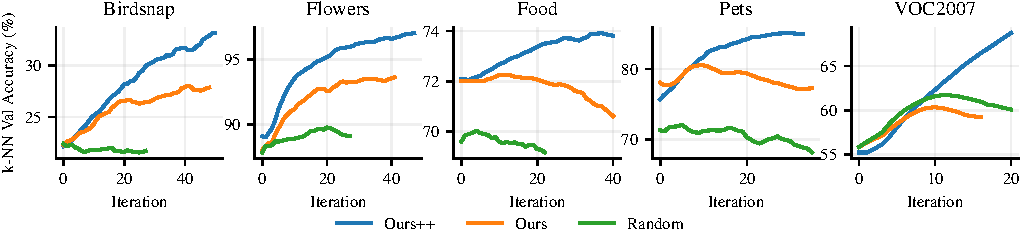
\includegraphics[width=\linewidth]{figures/ssl-curves-updated.pdf}
    \caption{\textbf{Learning curves in self-supervised setting.} $k$-NN validation accuracy improves across iterations on each target dataset. Without using any labels, Internet Explorer identifies and focuses on relevant concepts for each target dataset. This allows it to find more useful data than the baseline that searches for random concepts. Adding GPT-generated descriptors (Ours++) further improves performance by enabling Internet Explorer to generate diverse views of useful concepts. 
    % Interestingly, the random baseline does quite well on VOC2007, perhaps because coarse-grained classification benefits from a broader variety of training data. 
    } 
    \label{fig:learning_curves}
\end{figure*}

\begin{figure*}[t]
    \centering
    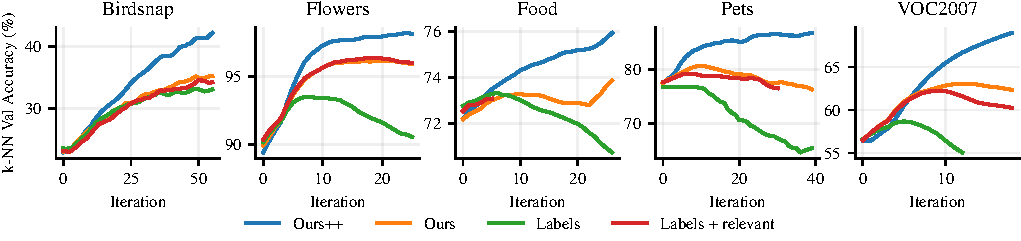
\includegraphics[width=\linewidth]{figures/semisup-curves-updated.pdf}
    \vspace{-0.3in}
    \caption{\textbf{Learning curves in label set-guided setting.} Using knowledge of the label set improves the performance of all methods. Internet Explorer (Ours) outperforms the baselines on all datasets, and adding GPT-generated descriptors (Ours++) further improves performance.
    }
    \label{fig:semisup_learning_curves}
    % \vspace{-0.05in}
\end{figure*}


\subsection{Label Set-guided Exploration}
% explain why this setting is also potentially practical 
% explain the baselines 
In practice, we may sometimes know the set of labels for our task even if we do not have image-label pairs (\ie, the English names of the classes).
For example, we may know that our data contains images of ``Golden Retrievers,'' ``Maine Coon,'' \etc, even if we do not have any images labeled with these names.
Knowing the label set greatly accelerates learning on the Internet, because it acts as a strong prior on what could be useful for our target dataset and allows us to focus our exploration on the subset of the vocabulary that is most likely to be useful.
Using our text similarity model, we reduce the size of the vocabulary by selecting the top 
% 10,000 concepts
$10\%$ ($14{,}635$ concepts)
with the largest average top-$k$ similarity to the label set in text embedding space. We set $k$ to a third of the size of the label set to reduce the impact of outliers.
Restricting our vocabulary to a semantically relevant subset also strengthens our baselines by ensuring that they only search for potentially useful concepts.

We compare 4 methods in this setting:
\begin{enumerate}[noitemsep,topsep=0pt]
    \item Labels: only search for labels. 
    \item Labels + relevant: search for labels half of the time, and random concepts from the pruned vocabulary the other half of the time. 
    \item Ours: sample labels half of the time and sample from our learned concept distribution the other half. 
    \item Ours++: additionally use GPT-generated descriptors.
\end{enumerate}
We call this setting ``label set-guided,'' since we have additional supervision in the form of the label set.

% \subsection{Datasets and Metrics}
\subsection{Datasets}
We evaluate Internet Explorer on 4 popular small-scale fine-grained classification datasets: Birdsnap~\cite{berg2014birdsnap}, Flowers-102~\cite{nilsback2008automated}, Food101~\cite{bossard2014food}, and Oxford-IIT Pets~\cite{parkhi2012cats}.
% which are commonly used to evaluate transfer learning for large pre-trained models~\cite{kornblith2019better}. 
We also evaluate on Pascal VOC 2007 (Classification)~\cite{everingham2010pascal}---a coarse-grained multi-label classification task consisting of only $2{,}040$ training examples, making it ideal for testing whether Internet Explorer can efficiently find relevant useful data.
We do not target large-scale datasets like ImageNet~\cite{deng2009imagenet} because they already contain over a million human-curated Internet images.
% We compare the representation quality of our model \wrt~its target dataset using two metrics: $k$-nearest neighbors ($k$-NN) accuracy and linear probe accuracy. 
% $k$-NN accuracy can be computed quickly, so we use this to plot learning curves of model performance after every iteration during training. We report the early-stopped linear probe accuracy in our tables.

\subsection{Evaluation Metrics}
We compare the representation quality of our models using two metrics: k-nearest neighbors (k-NN) accuracy  and linear probe accuracy. To measure k-NN accuracy, we use our ResNet-50 to encode each dataset's training and test sets. Then, for each test example, we find its $k$ nearest neighbors in representation space and use the mode of its neighbors' labels as the prediction. We use k-NN accuracy to plot learning curves of model performance after every iteration, since it is easy to quickly compute.

To compute the linear probe accuracy, we first select the best-performing model over all iterations on the validation set according to the k-NN accuracy. Then, we learn a linear head on top of these learned representations by minimizing the cross-entropy loss. We tune the weight decay parameter in the logscale range $(10^{-6}, 10^6)$, as is done in~\cite{radford2021learning}, using \texttt{scikit-learn}~\cite{pedregosa2011scikit} with Brent's method~\cite{brent1973algorithms}.


\begin{table}[t]
    \centering
    \begin{adjustbox}{width=1\textwidth}
    \begin{tabular}{lc@{\hskip 0.12em}cc@{\hskip 0.12em}cc@{\hskip 0.12em}cc@{\hskip 0.12em}cc@{\hskip 0.12em}cc@{\hskip 0.12em}cc@{\hskip 0.12em}cc}
    \toprule
        % Model & Flowers102 & Food101 & Stanford Cars & Oxford-IIIT Pets & Total Images & GPU-hours \\
        Model & \multicolumn{2}{l}{Birdsnap} & \multicolumn{2}{l}{Flowers} & \multicolumn{2}{l}{Food}  & \multicolumn{2}{l}{Pets} & \multicolumn{2}{l}{VOC2007} & Images & GPU hrs. \\
    \midrule
    % \textit{Fixed dataset, language supervision} \\
    \textit{Fixed dataset, lang. supervision} \\
        \;\;\;CLIP ResNet-50 (\textbf{oracle})  & $57.1$ & & $96.0$ & & $\bf{86.4}$ & & $88.4$ & & $\bf{86.7}$ & & $400 \times 10^6$ & $4{,}000$ \\ % 82.8 for CLIP pascal 
    \midrule
    \textit{Fixed dataset, self-supervised} \\
        \;\;\;MoCo-v3 (ImageNet pre-train)  & $26.8$ & & $83.2$ & & $70.5$ & & $79.6$ & & $-$ & &  $1.2 \times 10^6$ & $72$ \\
        %\;\;\; MoCo-v3 (target only)                      & 80.0 & 0    & 0    & $< 10^5$ & 2 \\
        \;\;\;MoCo-v3 (ImageNet + target)  & $39.9$ & & $94.6$ & & $78.3$ & & $85.3$ & & $58.0^\dag$ & & $1.2 \times 10^6$ & $72 + 12$ \\
    \midrule
    \textit{No label set information} \\
        \;\;\;Random exploration  & $39.6$ & \red{$(-0.3)$} & $95.3$ & \green{$(+0.7)$} & $77.0$ & \red{$(-1.3)$} &  $85.6$ & \green{$(+0.3)$} & $70.2$ & \green{$(+12.2)$} &  $2.2 \times 10^6$ & $84 + 40$ \\
        \;\;\;Ours  & $43.4$ & \green{$(+3.5)$} & $97.1$ & \green{$(+2.5)$} & $80.5$ & \green{$(+2.2)$} & $86.8$ & \green{$(+1.5)$} & $68.5$ & \green{$(+10.5)$}  & $2.2 \times 10^6$ & $84 + 40$ \\
        \;\;\;Ours++  & $54.4$ & \green{$(+14.5)$} & $98.4$ & \green{$(+3.8)$} & $82.2$ & \green{$(+3.9)$} & $89.6$ & \green{$(+4.3)$} & ${80.1}$ & \green{${(+22.1)}$} & $2.2 \times 10^6$ & $84 + 40$ \\
    \midrule 
    \textit{Use label set information} \\       
        \;\;\;Search labels only  & $47.1$ & \green{$(+7.2)$} & $96.3$ & \green{$(+1.7)$} & $80.9$ & \green{$(+2.6)$} & $85.7$ & \green{$(+0.4)$} & $61.8$ & \green{$(+3.8)$} & $2.2 \times 10^6$ & $84 + 40$ \\
        \;\;\;Labels + relevant terms  & $49.9$ & \green{$(+10.0)$}& $98.0$ & \green{$(+3.4)$} & $81.2$ & \green{$(+2.9)$} & $87.0$ & \green{$(+1.7)$} & $67.5$ & \green{$(+9.5)$} & $2.2 \times 10^6$ & $84 + 40$ \\
        \;\;\;Ours  & $52.0$ & \green{$(+12.1)$} & $97.6$ & \green{$(+3.0)$} & $81.2$ & \green{$(+2.9)$} & $87.3$ & \green{$(+2.0)$} & $70.3$ & \green{$(+14.3)$} & $2.2 \times 10^6$ & $84 + 40$ \\
        \;\;\;Ours++  & $\mathbf{62.8}$ & \green{$\mathbf{(+22.9)}$} & $\bf{99.1}$ & \green{$\mathbf{(+4.5)}$} & $84.6$ & \green{$(+6.3)$} & $\mathbf{90.8}$ & \green{$\mathbf{(+5.5)}$} & ${79.6}$ & \green{$(+21.6)$} & $2.2 \times 10^6$ & $84 + 40$ \\
    \bottomrule
    \end{tabular}
    \end{adjustbox}
    % \caption{\textbf{Linear probe accuracy on targeted datasets}.}
    \caption{\textbf{Linear probing accuracy}. Our method significantly improves the starting checkpoint performance in just 40 additional hours of training. We show the performance change from the starting MoCo-v3 (ImageNet + target) initialization in \green{green}/\red{red}. CLIP numbers correspond to linear probe (which is higher than its zero-shot accuracy). Internet Explorer reaches or often surpasses CLIP (oracle with 2x params) performance on each dataset while using 2.5\% as much compute and 0.5\% as much data. ${}^{\dag}$For VOC2007, we do not do ImageNet pre-training because ImageNet is too close to VOC2007.
    % obscures the effect of Internet Explorer. 
    % We report $k$-NN accuracy in the VOC2007 column and show LP in the supplementary. 
    }
    \label{tab:main_results}
\end{table}


\begin{figure}[t]
\centering
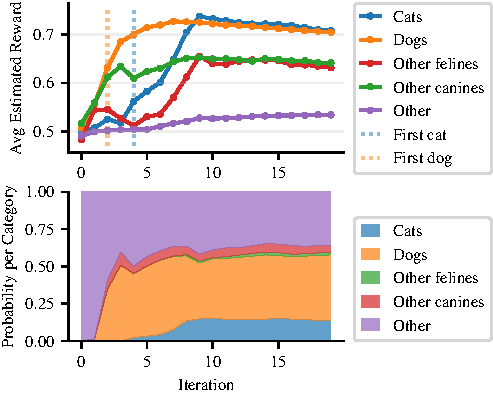
\includegraphics[width=0.675\linewidth]{figures/pets_ssl_reward_over_training2.pdf}
\caption{\textbf{Self-supervised concept discovery on Pets dataset.} When targeting the Pets dataset, self-supervised Internet Explorer quickly estimates high reward for concepts from the cat category (82 concepts) and dog category (246 concepts). It is also able to identify felines that are not cats (e.g., tigers) and canines that are not dogs (e.g., wolves), although it gives them lower reward on average. Finding these categories is especially challenging, since they comprise only $460/146{,}347 = 0.3\%$ of the vocabulary.}
\label{fig:reward_over_training}
\end{figure}



\begin{figure*}[t]
    \centering
    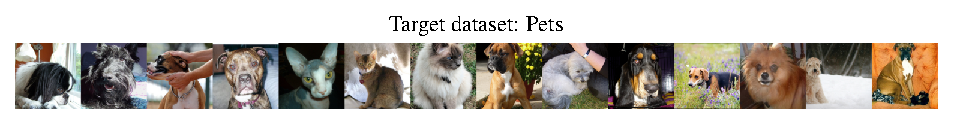
\includegraphics[width=\linewidth]{figures/pets_targets.pdf}\\
    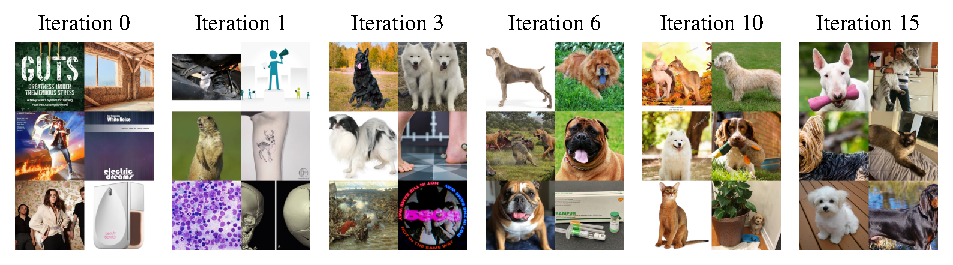
\includegraphics[width=\linewidth]{figures/pets-progression-962-2col-3row.pdf}
    % 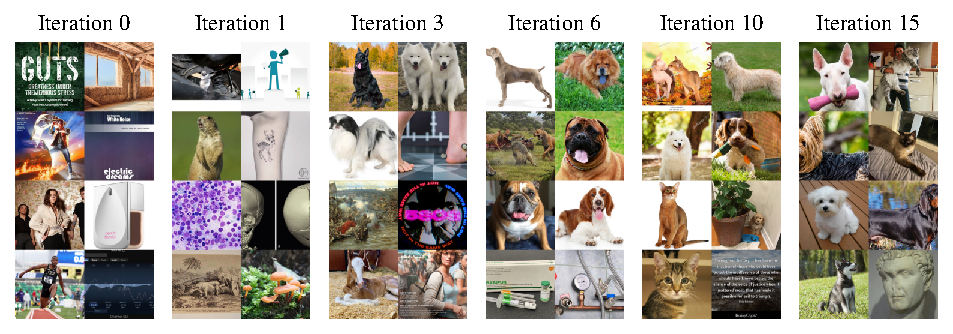
\includegraphics[width=\linewidth]{figures/pets-progression-962-2col.pdf}
    \caption{
    % \textbf{Progression of downloaded images over training.} The top row shows the target distribution and the bottom ones show the sets of images queried by our Internet Explorer. As the progression goes on, the image set discovered by the Internet Explorer starts to more closely resemble the target dataset distribution.
    \textbf{Progression of downloaded images across training.} \textbf{Top:} samples of Oxford-IIIT Pets images.\ \textbf{Bottom:} samples of images queried by Internet Explorer across iterations. As the method learns, it makes queries that are progressively more relevant to the target dataset.
    }
    \label{fig:progression}
    \vspace{-0.15in}
\end{figure*}

\section{Results and Analysis}
\subsection{Self-supervised Results}
\cref{fig:learning_curves} shows how Internet Explorer improves the $k$-NN accuracy more efficiently than sampling queries uniformly at random from the concept vocabulary. In fact, random sampling occasionally decreases accuracy, likely due to the fact that Internet images can generally be unsuitable for pre-training due to issues such as watermarks, images containing text, and overly photogenic images~\cite{mezuman2012learning,chen2015webly}. \cref{tab:main_results} shows that our method significantly improves on the starting MoCo-v3 (ImageNet + target) checkpoint and can outperform a CLIP~\cite{radford2021learning} model of the same size while using much less compute and data. This is impressive as CLIP can be thought of as an oracle, since its training set contains up to 20k Bing image search results for each WordNet lemma (in addition to other queries).
Using GPT-generated descriptors in ``Ours++'' also significantly improves performance by enabling Internet Explorer to generate diverse views of the most useful concepts. 
% We show example image results with and without descriptors in the supplementary. 

\subsection{Self-supervised Exploration Behavior}
\label{sec:exploration_behavior}
\cref{fig:reward_over_training} shows the progression of Internet Explorer (Ours++) behavior on the Pets dataset in the self-supervised setting. Since Pets consists of cat and dog breeds, to analyze the results, we use the WordNet hierarchy to divide concepts in our vocabulary into 5 meaningful categories: cats, dogs, non-cat felines (e.g., lion), non-dog canines (e.g., wolf), and other. This categorization is only done for this post hoc analysis and is not provided during training. \cref{fig:reward_over_training} (top) shows that
% the average estimated reward within each category across the first 20 iterations of training, and the bottom one shows how much probability mass each category has. 
Internet Explorer rapidly identifies the roughly $0.3\%$ of concepts that are useful for Pets. During the first two iterations, the average estimated reward for each category is roughly the same. However, after the first dog concept is searched in iteration $\#2$, the estimated reward and probability mass for dogs and other canines rapidly increases. The same happens for cats after the first cat is searched in iteration $\#4$. Interestingly, while ``other felines'' and ``other canines''  have higher average reward than the ``other'' category, they still have much lower reward than cats and dogs. This indicates that our model understands that other felines and canines (mostly large, wild predators) are only moderately relevant for house pet cats and dogs. 

\cref{fig:progression} shows how Internet Explorer downloads progressively more useful images over time. It shows 8 random images that were downloaded in iteration $\#0$, $\#1$, $\#3$, $\#6$, $\#10$, and $\#15$. Iteration $\#0$ contains mostly useless data, like graphics or screenshots, but Pets-relevant images already make up most of the downloads by iteration $\#3$. 
Results for other datasets are shown in \cref{sec:progression_continued}.

\subsection{Label Set-guided Results}
% As discussed earlier, we now make use of the label set of the target dataset without knowing the exact image-label mapping. 
Internet Explorer significantly outperforms the stronger baselines in the label set-guided setting where we additionally have knowledge of the label set. Searching for the label set continuously provides useful data and helps us rapidly identify other useful concepts. Together with the diversity promoted by GPT descriptors, Ours++ outperforms CLIP in 3/5 datasets and approaches its performance in the other 2, using just 2.5\% of the time and 0.5\% the data---as can be seen in \cref{tab:main_results}. The fact that Ours++ can match/outperform CLIP is especially impressive, since CLIP has access to up to 20k Bing image search results for each WordNet lemma (in addition to other queries).
k-NN accuracy learning curves for the label set-guided setting are shown in \cref{fig:semisup_learning_curves}.

% Note that we train Internet Explorer from scratch on VOC2007 and do not use an ImageNet pre-trained MoCo-v3 model as initialization. 
% Note that we train from scratch on VOC2007 and do not do ImageNet pre-training because ImageNet's similarity to VOC2007 obscures the effect of Internet Explorer.

\subsection{Learning from other sources of data}
\label{subsec:search_engine_main}

Google Images is an exceptionally useful data source for Internet Explorer. It offers access to a large portion of the Internet's images, and it ranks images using weak supervision from the image caption, surrounding text, click rates, image features, incoming and outgoing hyperlinks, and other signals. This extra supervision is helpful and should be utilized. Nonetheless, we show that Internet Explorer is agnostic to the choice of text-to-image search engine and can still rapidly improve even when the data source is much noisier. 

\begin{table*}[h]
    \centering
    \begin{adjustbox}{width=1\textwidth}
    \begin{tabular}{@{\extracolsep{4pt}}lccccccccc}
    \toprule
        % Model & Flowers102 & Food101 & Stanford Cars & Oxford-IIIT Pets & Total Images & GPU-hours \\
        \multirow{2}{*}{\textbf{Model}}
        &\multicolumn{3}{c}{\textbf{Flowers}} 
        &\multicolumn{3}{c}{\textbf{Food}}
        &\multicolumn{3}{c}{\textbf{Pets}} \\
        \cmidrule{2-4} \cmidrule{5-7} \cmidrule{8-10}
        
        
        & Google & Flickr & LAION & Google & Flickr & LAION & Google & Flickr & LAION \\
    \midrule
    \textit{Fixed dataset} &&&&&&&&&\\    
        \;\;\; MoCo-v3 (IN)                          & $83.2$ & $83.2$ & $83.2$ & $70.5$ & $70.5$ & $70.5$ & $79.6$ & $79.6$ & $79.6$ \\
        \;\;\; MoCo-v3 (IN + target)                 & $94.6$ & $94.6$ & $94.6$ & $78.3$ & $78.3$ & $78.3$ & $85.3$ & $85.3$ & $85.3$ \\
    \midrule
    \textit{Undirected search} &&&&&&&&&\\    
        \;\;\;Random exploration                     &  $95.3$  &  $95.2$  &  $94.8$  &  $77.0$ &  $80.0$  &  $80.2$  &  $85.6$ & $84.4$  & $85.1$ \\
    \midrule 
    \textit{Internet Explorer} &&&&&&&&&\\    
        % \;\;\;Random exploration                      &    &    &    &    &    &    &    &    &    \\
        % \;\;\;Ours                                   &  ? &  ? &  ? &  ? &  ? \\
        \;\;\;Ours++ (no label set)                  &  $98.4$  &  $98.1$  &  $94.6$  &  $81.2$  &  $80.3$  &  $80.9$  &  $87.3$  &  $88.4$  &  $85.9$  \\
    % \midrule 
        % \;\;\;Search labels only                      &  ? &  ? &  ? &  ? &  ? \\
        % \;\;\;Labels + relevant                       &    &    &    &    &    &    &    &    &    \\
        % \;\;\;Ours                                    &  ? &  ? &  ? &  ? &  ? \\
        \;\;\;Ours++ (with label set)                &  $\bf{99.1}$ &  $\bf{99.0}$ &  $\bf{95.8}$ & $\bf{84.6}$ & $\bf{81.9}$  &  $\bf{81.0}$  & $\bf{90.8}$ &  $\bf{89.1}$  &  $\bf{86.7}$  \\
    \bottomrule
    \end{tabular}
    \end{adjustbox}
    \caption{\textbf{Linear probe accuracy with other search engines}. Internet Explorer improves its performance using any search engine, including Flickr and our custom text-based LAION search engine.}
    \label{tab:search_engine}
\end{table*}

\begin{figure*}[p]
    \centering
    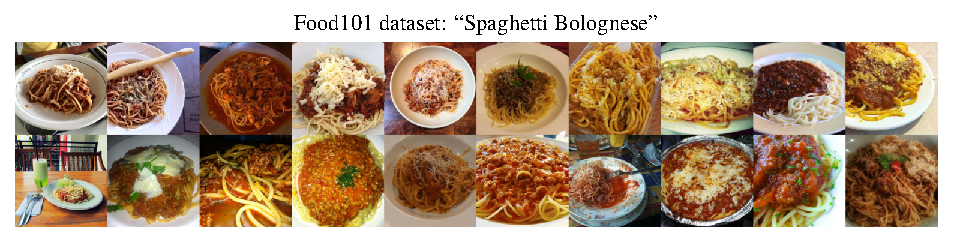
\includegraphics{figures/food-spaghetti.pdf} \\
    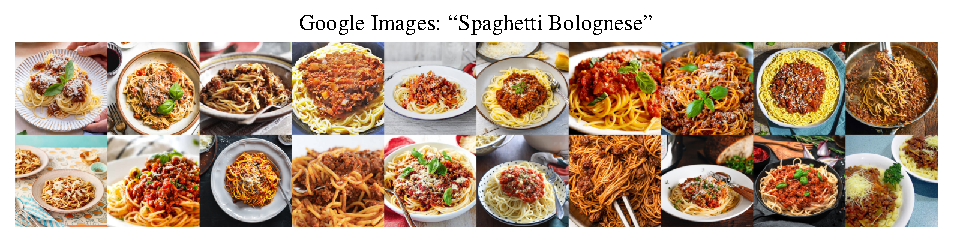
\includegraphics{figures/google-spaghetti.pdf} \\
    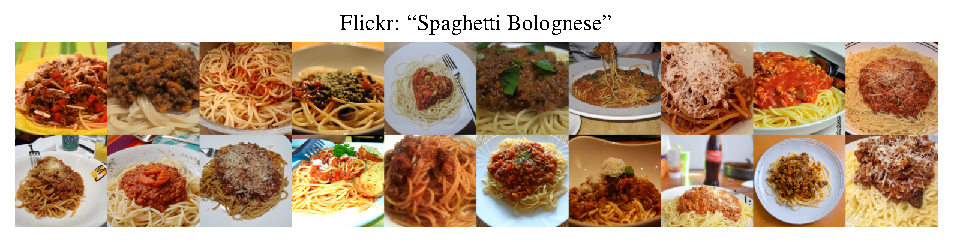
\includegraphics{figures/flickr-spaghetti.pdf} \\
    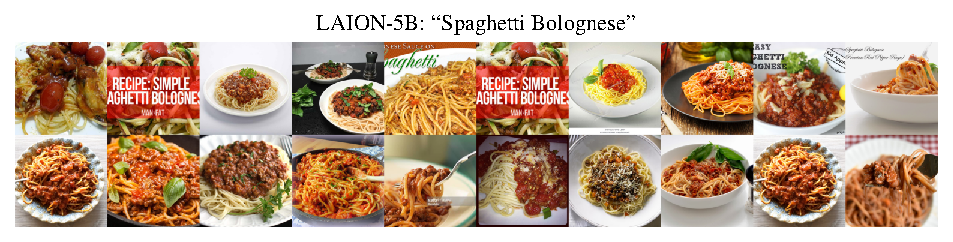
\includegraphics{figures/laion5b-spaghetti.pdf} 
    \caption{\textbf{Comparison of different search engines.} We show images for the ``spaghetti bolognese'' class in the Food101 dataset, as well as 20 search results for ``spaghetti bolognese'' from Google Images, Flickr, and LAION5B. Google images are typically well-lit, aesthetic food blog pictures. In comparison, Flickr images are messier, darker, and capture a wider variety of real-world conditions. LAION-5B images lie somewhere in the middle, but contain text overlays much more frequently. Duplicate image results are also common.}
    \label{fig:data_comparison}
\end{figure*}

\begin{wrapfigure}{R}{0.4\textwidth}
\centering
    \vspace{-2em}
    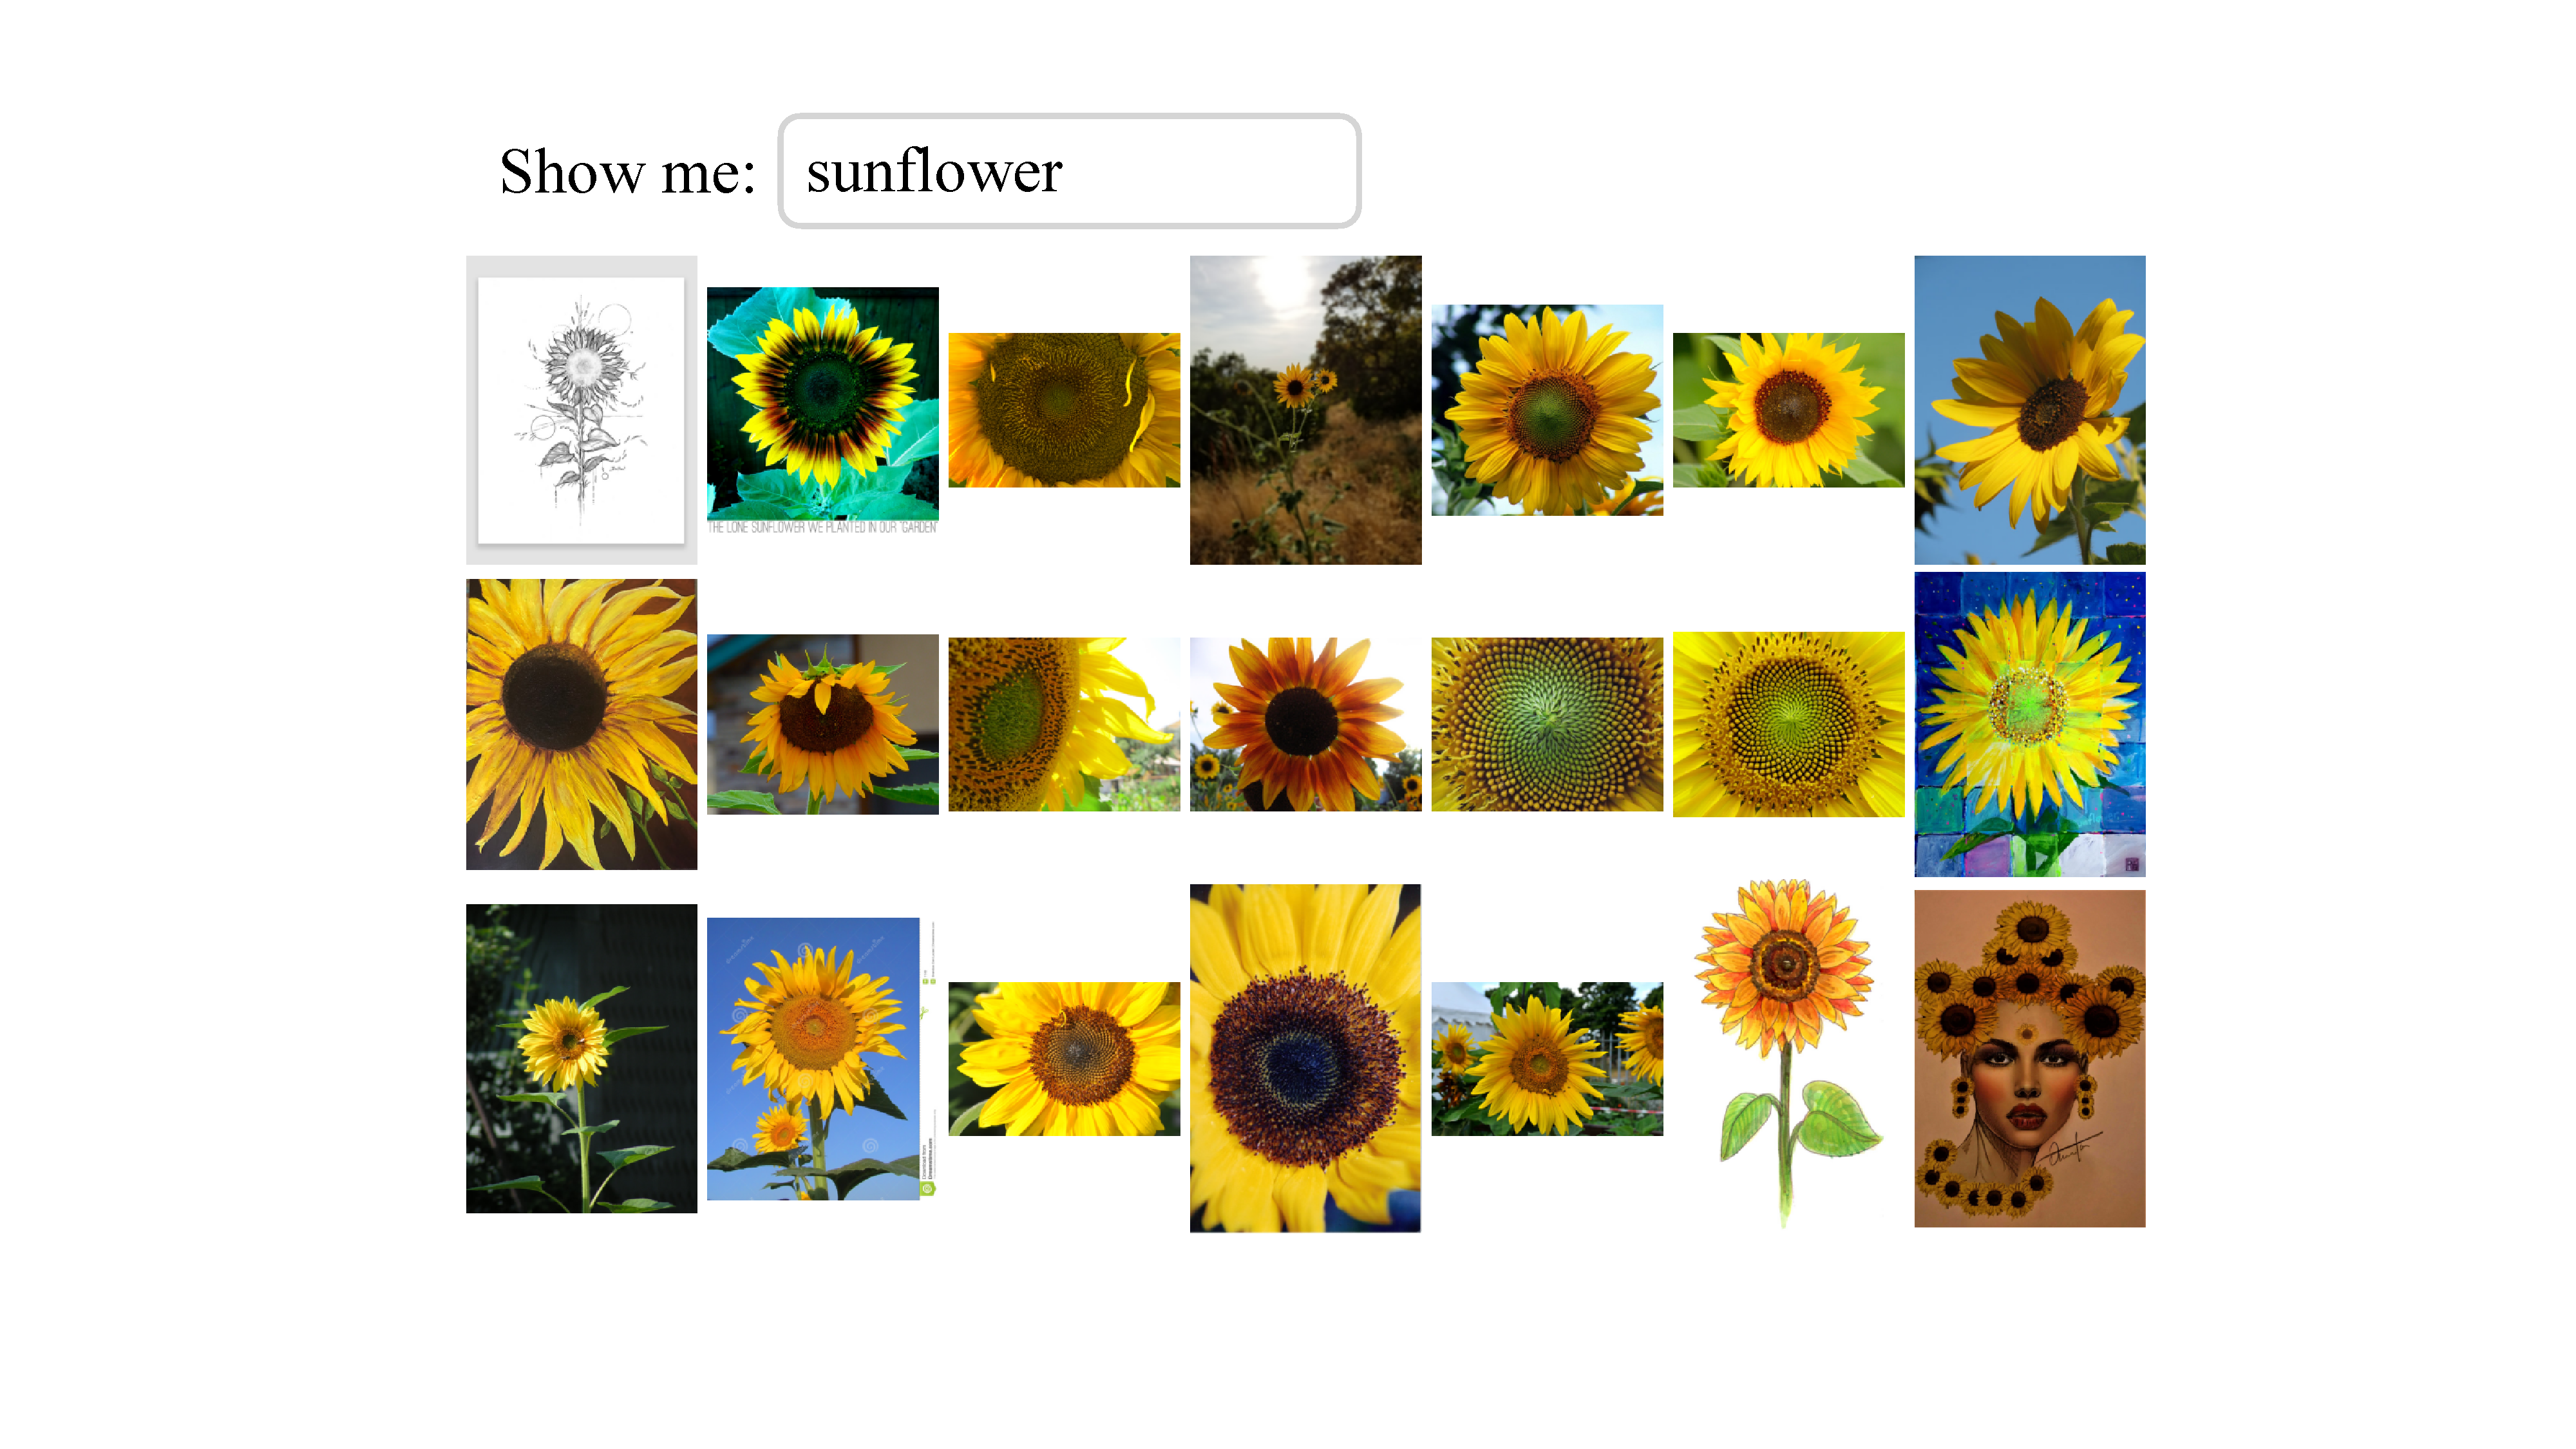
\includegraphics[width=\linewidth]{figures/laion_search_engine.pdf}
    \vspace{-1em}
    \caption{\textbf{Custom LAION-5B search engine.} We build a custom text-to-image search engine that finds images within the LAION-5B dataset by doing nearest neighbor search in text embedding space---using no image features whatsoever.}
    \label{fig:laion_search_engine}
    \vspace{-4em}
\end{wrapfigure}

To test Internet Explorer in the most minimal setting, we build a custom search engine that finds images solely using their accompanying text, without using any pre-trained visual features whatsoever. We use the LAION-5B dataset~\cite{schuhmann2022laion}, which consists of 5.85 billion noisy image-caption pairs. We filter the dataset to only include samples with English captions and images with at least $512^2$ pixels. This leaves us with about 600M text-image pairs. To find image results for a query, we find the 100 captions closest to the query in text representation space, then return the associated images.
We use a pre-trained text embedding model~\cite{reimers2019sentence} to compute 384-dimensional text embeddings for each caption. Then, we use Faiss~\cite{johnson2019billion} to compute a fast, approximate nearest-neighbors lookup index. Querying our custom search engine finds 100 image results in less than a second. \cref{fig:laion_search_engine} shows that our search engine is reasonably accurate, even without using any image features. 

We also test Flickr's photo search API as another text-to-image search engine, in addition to Google Images and LAION. \cref{fig:data_comparison} shows that each data source has its own tendencies. For the ``spaghetti bolognese'' query, Google Images is biased~\cite{mezuman2012learning,chen2015webly} towards brightly-lit, photogenic images that typically come from food blogs. Flickr mainly consists of amateur home photos, so it returns a messier variety of images that perhaps better capture the real world. LAION images come from web crawling, without any ranking, so they additionally contain many graphics with text overlays. The same image can also frequently show up in the LAION results multiple times, as a result of being posted on multiple separate pages. 


\begin{figure*}
    \centering
    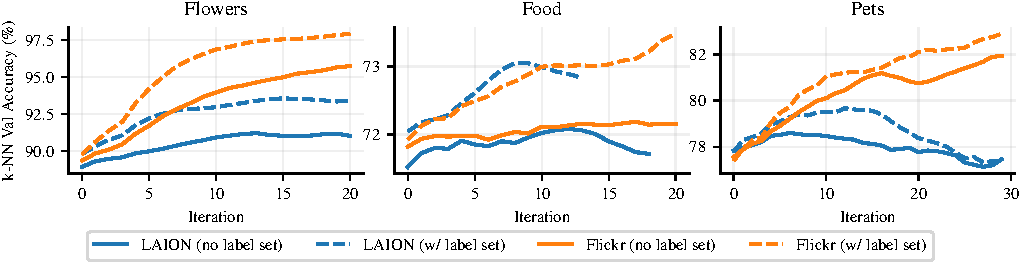
\includegraphics[width=\linewidth]{figures/laion-curves.pdf}
    \caption{\textbf{Learning from Flickr and LAION-5B.} Even with the noisy search results returned by Flickr and LAION, Internet Explorer still continuously improves performance. }
    \label{fig:other_data_curves}
\end{figure*}


\cref{fig:other_data_curves} and \cref{tab:search_engine} show that Internet Explorer consistently improves over time, regardless of the search engine we use. 
Google consistently does best, followed by Flickr, then LAION (which has the smallest pool of images to draw from).
Using Internet Explorer to search LAION-5B consistently performs \textit{better} than random exploration---indicating that Internet Explorer is effective even for selecting data from a static dataset.
Overall, these results are proof that Internet Explorer can effectively utilize any window into the Internet's vast ocean of image data. 


\subsection{Are we finding the entire test set online?}
\label{sec:finding_test_set_online}

\newcommand{\blue}[1]{\textcolor{Cerulean}{#1}}
\begin{table}[t]
    \centering
    % \begin{tabular}{lccccccccc}
        \begin{adjustbox}{width=1\textwidth}
        \begin{tabular}{
            lr@{\hskip 0.12em}
            rr@{\hskip 0.12em}
            rr@{\hskip 0.12em}
            rr@{\hskip 0.12em}
            rr@{\hskip 0.12em}
            rc}
        \toprule
            % Model & Flowers102 & Food101 & Stanford Cars & Oxford-IIIT Pets & Total Images & GPU-hours \\
            % Model & Birdsnap & Flowers & Food  & Pets & VOC2007  & Images Downloaded \\
            &
            \multicolumn{2}{l}{Birdsnap} & 
            \multicolumn{2}{l}{Flowers} & 
            \multicolumn{2}{l}{Food} & 
            \multicolumn{2}{l}{Pets} & 
            \multicolumn{2}{l}{VOC2007} \\
        \midrule
        Target test set size                          &  \multicolumn{2}{l}{$1849$} &  \multicolumn{2}{l}{$6142$} & \multicolumn{2}{l}{$25246$} &\multicolumn{2}{l}{$3663$} &\multicolumn{2}{l}{$4952$} \\ 
        % Target test set size                          &  \multicolumn{2}{c}{$1849$} &  \multicolumn{2}{c}{$6142$} & \multicolumn{2}{c}{$25246$} &\multicolumn{2}{c}{$3663$} &\multicolumn{2}{c}{$4952$} & $-$ \\ 
        \midrule
        \textit{No exploration} \\
            \;\;\; Target training set overlap                          &  $1$ & \blue{$(0.05\%)$} &  $5$ & \blue{$(0.01\%)$}& $34$ & \blue{$(0.13\%)$} & $21$ & \blue{$(0.57\%)$} &  $0$ & \blue{$(0.00\%)$} \\
        \midrule
        % \textit{No label set information} \\
        \textit{Internet Explorer} \\
            % \;\;\;Random exploration                     &  ? &  ? &  ? &  ? &  ? \\
            % \;\;\;Ours                                   &  ? &  ? &  ? &  ? &  ? \\
            % \;\;\;Ours++ (no label set)                         &  $28/1849$ & & $11/6142$ & & $35/25246$ & & $26/3663$ & & $1/4952$ & & $\approx 10^6$\\
            \;\;\;Ours++ (no label set)                         &  $28$ & \blue{$(+1.46\%)$} & $11$ & \blue{$(+0.01\%)$} & $35$ & \blue{$(+0.00\%)$} & $26$ & \blue{$(+0.14\%)$}& $1$ & \blue{$(+0.02\%)$} \\
        % \midrule 
        % \textit{Use label set information} \\       
            % \;\;\;Search labels only                      &  ? &  ? &  ? &  ? &  ? \\
            % \;\;\;Labels + semantically relevant terms    &  ? &  ? &  ? &  ? &  ? \\
            % \;\;\;Ours                                    &  ? &  ? &  ? &  ? &  ? \\
            \;\;\;Ours++ (with label set)                       & $57$ & \blue{$(+3.03\%)$} & $27$ & \blue{$(+0.36\%)$}& $35$ &\blue{$(+0.00\%)$} & $43$ &\blue{$(+0.60\%)$} & $1$ &\blue{$(+0.02 \%)$} \\
    \bottomrule
\end{tabular}
\end{adjustbox}
    \caption{
        \textbf{Number of leaked test set images}. We use image hashing to compute the fraction of test images present in the set of images downloaded by Internet Explorer. 
        % We show (number of leaked images)$/$(number of unique test images).
        Surprisingly, the training/validation sets of these datasets already leak a small fraction of the test sets---Pets is the most egregious, with $0.57\%$ of test images leaked.
        For each dataset, we show the test set size, the number of leaked test images, and the percentage of the test set that this represents in \blue{blue}; for each version of our method, we show the total number of leaked images that the model had access to, and the percentage increase this represents over the dataset's leakage in \blue{blue}.
        Leakage numbers for our methods include this train-test leakage, since our methods also train on the target dataset's training set. Internet Explorer only finds a tiny fraction of test set images online, and it only uses them for self-supervised training, so there is no \textit{label leakage}. Overall, Internet Explorer's increase in accuracy cannot be explained by test set leakage, so it must be improving performance through better feature learning and generalization.
    }
    \label{tab:leakage}
\end{table}
One may be concerned that Internet Explorer improves performance mainly by finding a significant portion of the test set images online. We address this concern by checking how much test data Internet Explorer has downloaded. We use difference hashing (dHash)~\cite{imagehash} to compute hashes for the target dataset's training set, its test set, and the $\approx 10^6$ images that Internet Explorer has downloaded. We compare hashes to determine how many test images were leaked, and we report the number of collisions in \cref{tab:leakage}. Across all five datasets, Internet Explorer finds very few test images. On Birdsnap, Internet Explorer finds 56 additional test set images that were not leaked in the training set, which is roughly $3\%$ of the test set. On the other datasets, the amount leaked ranges from $0.003\%$ to $0.6\%$ of the test set. Additionally, we only perform self-supervised training on downloaded images, so it is much harder for our model to cheat with the leaked images. Overall, given that Internet Explorer outperforms its starting checkpoint by between 5 to 30 percentage points, we conclude that its performance cannot be explained by cheating.
% we actually view it as a positive that Internet Explorer finds some test set images, because it means that it is learning to search for relevant images --- the MOST relevant images possible would be those from the dataset itself!
% Q: how do I segue to the above point?
% A: I think you can just say that it's a positive that IE finds some test set images, because it means that it is learning to search for relevant images --- the MOST relevant images possible would be those from the dataset itself!
% ok say it below:

In fact, we view it as a positive that Internet Explorer finds some test set images, because it serves as confirmation that it is learning to search for relevant images---and the most relevant images possible would be those from the dataset itself!
% beyond test imgs, Int exp finds a lot of internet images that are very relevant to the dataset.
% we now visualize the online images obtained, by providing examples of the top-10 most similar online images given a test set image.
% We use CLIP ViT-L/14 to compute the representations of the test set images, as well as the downloaded images
But beyond test set images, Internet Explorer finds a lot of internet images that are very relevant to the dataset. We visualize the top-10 most similar images for 5 randomly selected test set images from the Flowers, Food, and Pets datasets in \cref{fig:online_images}.  We use CLIP ViT-L/14 to compute the representations of the test set images, as well as the downloaded images. We then find the top-10 most similar online images given a test set image (from the downloaded images using Ours++ (with label set)).
We see that Internet Explorer finds several images that are very similar but not identical to the test set images.

% figures/internet-nns/flowers.png figures/internet-nns/food.png figures/internet-nns/pets.png figures/internet-nns/voc.png
\begin{figure}[p]
    \centering
    
    \begin{subfigure}{\textwidth}
        \centering
        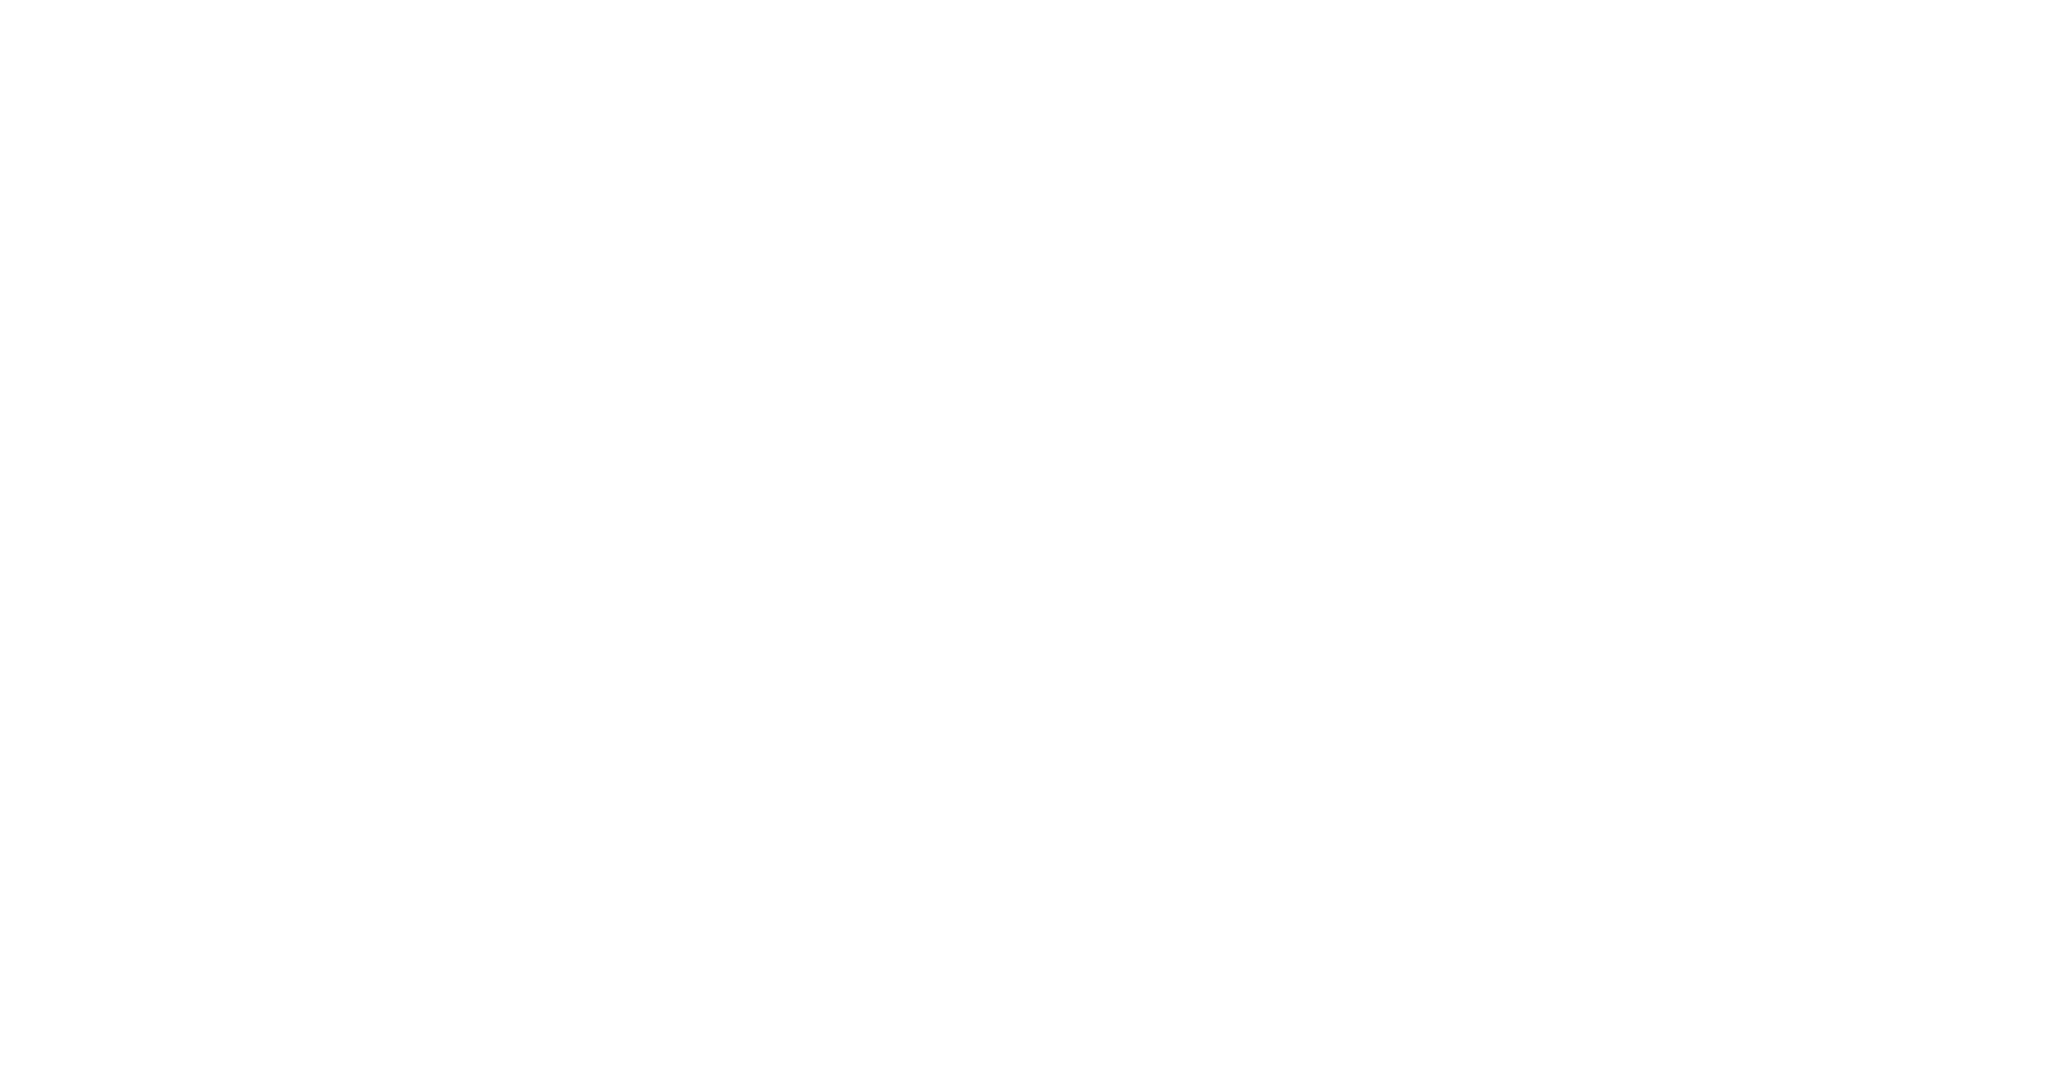
\includegraphics[width=0.75\textwidth]{figures/internet-nns/flowers.png}
        % \caption{Flowers}
        % \label{fig:flowers}
    \end{subfigure}
    \vspace{0.1em}

    \begin{subfigure}{\textwidth}
        \centering
        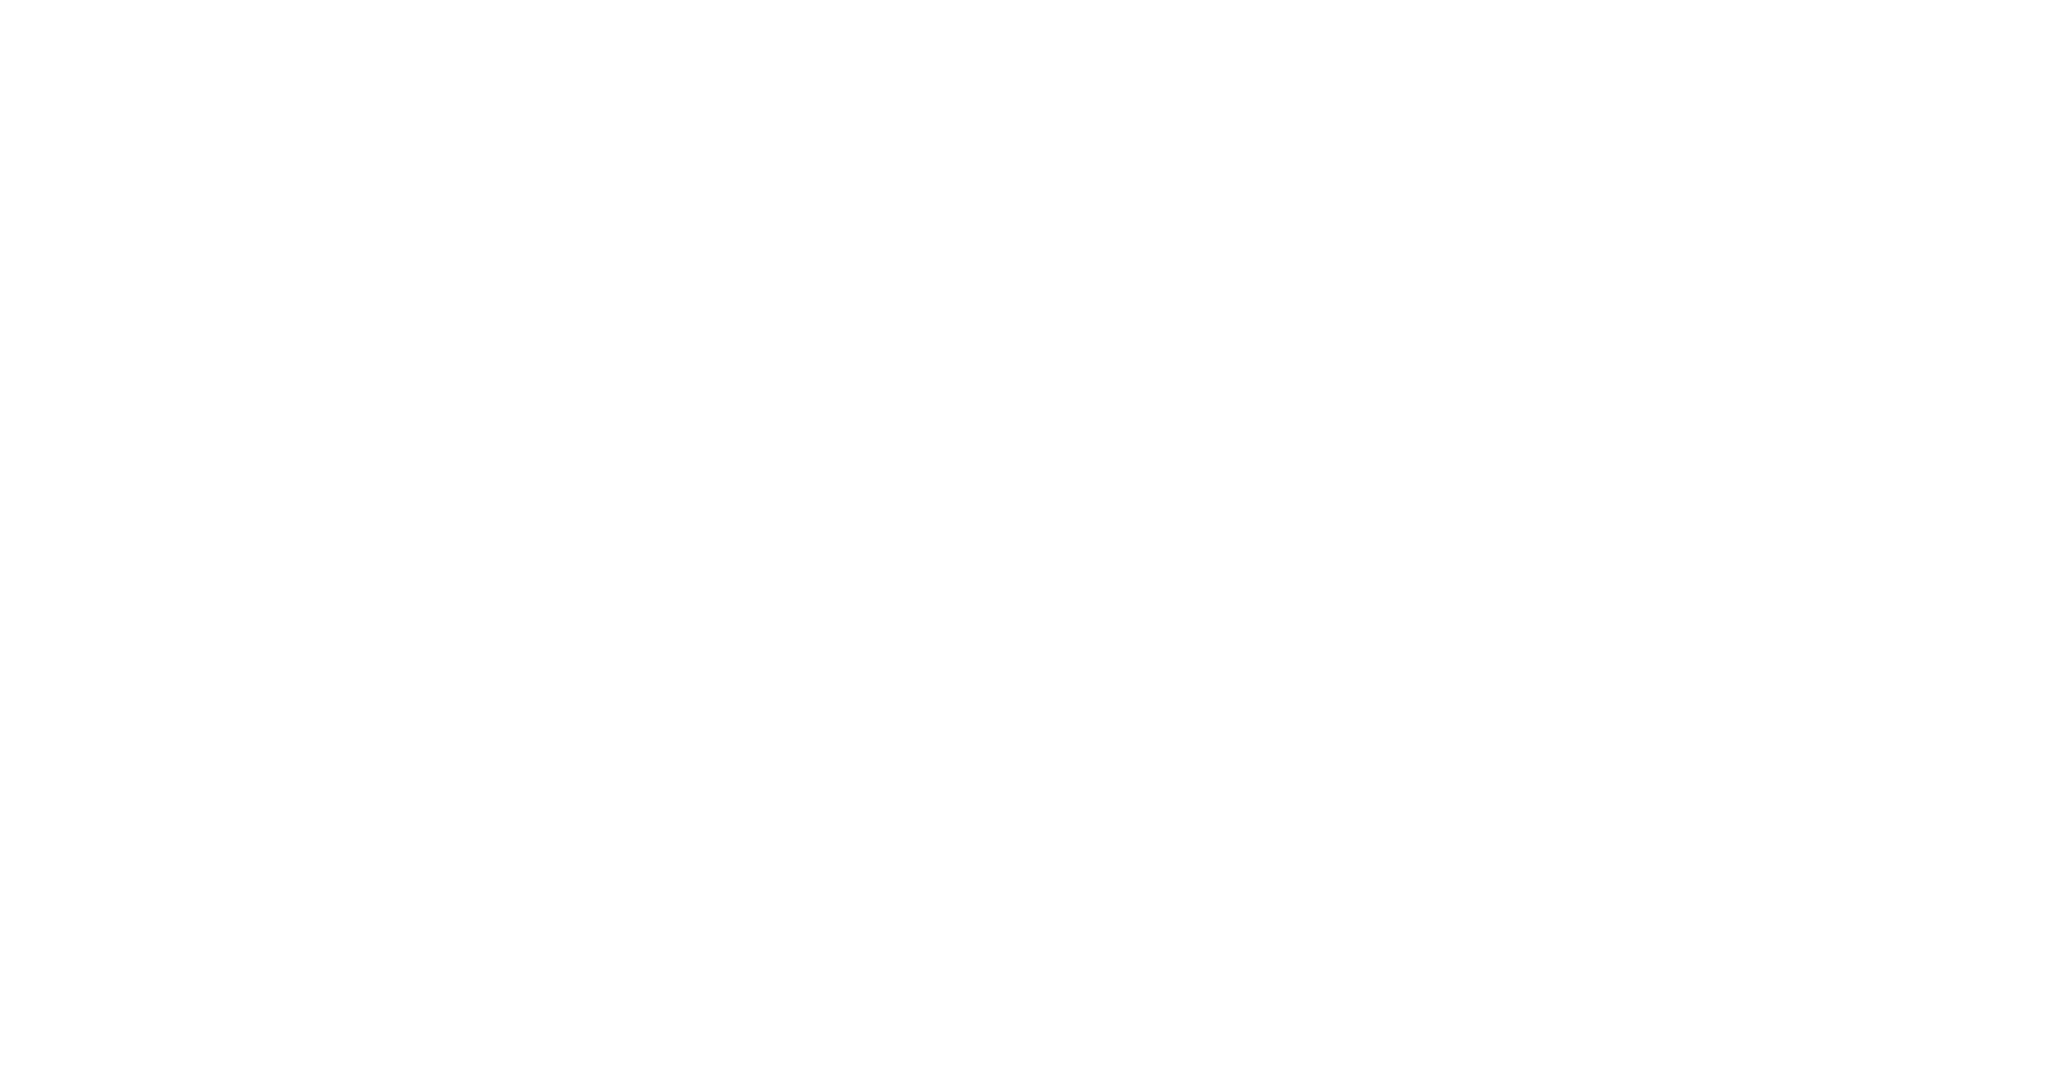
\includegraphics[width=0.75\textwidth]{figures/internet-nns/food.png}
        % \caption{Food}
        % \label{fig:food}
    \end{subfigure}
    \vspace{0.1em}

    \begin{subfigure}{\textwidth}
        \centering
        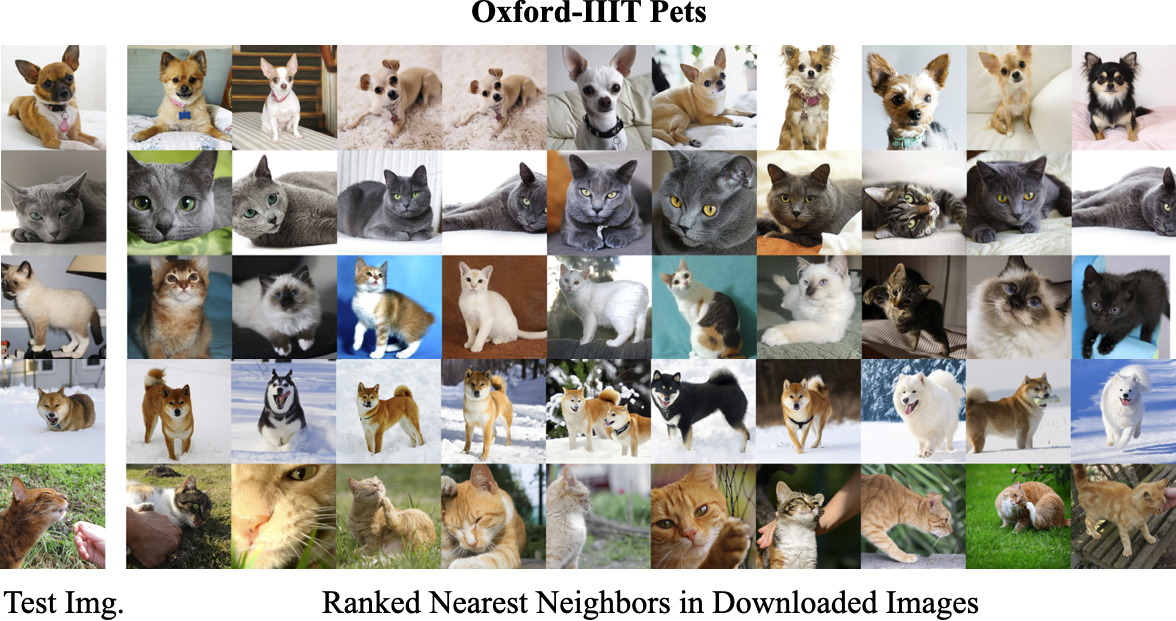
\includegraphics[width=0.75\textwidth]{figures/internet-nns/pets.png}
        % \caption{Pets}
        % \label{fig:pets}
    \end{subfigure}
    \vspace{0.1em}
    
    \caption{
        \textbf{Top-10 most similar online images}.
        The left column shows randomly chosen test set images from each dataset, and the right block shows the 10 most similar images in the downloaded data for each test image,
        ranked left to right.
        % ranked left to right in decreasing order of similarity and deduplicated (relative to other downloaded images, not the test images).
    }
    \label{fig:online_images}
\end{figure}

\subsection{Effect of image reward type}
\label{subsec:reward_analysis}
We run an ablation on the type of image relevance reward. Instead of calculating the image reward based on the average similarity to the $k=15$ nearest neighbors in representation space (as in \cref{subsec:ssl}), we also try using $k=1$ or the MoCo contrastive loss as the reward. Table~\ref{tab:image_reward} compares these three metrics in the label set-guided setting and shows that $k=15$ does best. We explain this result by qualitatively comparing the behavior of various metrics on Food101 in \cref{fig:reward_ranking} in the appendix. The MoCo loss does not identify relevant concepts, instead preferring images that are difficult to align across augmentations. Representation similarity with $k=1$ also fails, as it prefers images of zebras and text because these images are highly similar to a few outlier images in Food101. Our proposed reward with $k=15$ eliminates the influence of outliers and avoids this problem.

\begin{table}[h]
    \centering
    \begin{tabular}{lcc}
        \toprule
        Reward Type & Food \\
        \midrule
        MoCo loss & 81.2 \\
        1-NN sim  & 83.2 \\
        15-NN sim (ours) & \textbf{84.6} \\
        \bottomrule
    \end{tabular}
    \caption{\textbf{Ablation on type of image reward.}
    % We compare LP accuracy of 3 different rewards on Food in the label set-guided setting.
    MoCo loss does not identify relevant concepts, and $k=1$ similarity is too noisy to identify useful concepts. }
    \label{tab:image_reward}
\end{table}

\begin{figure}[h]
    \centering
    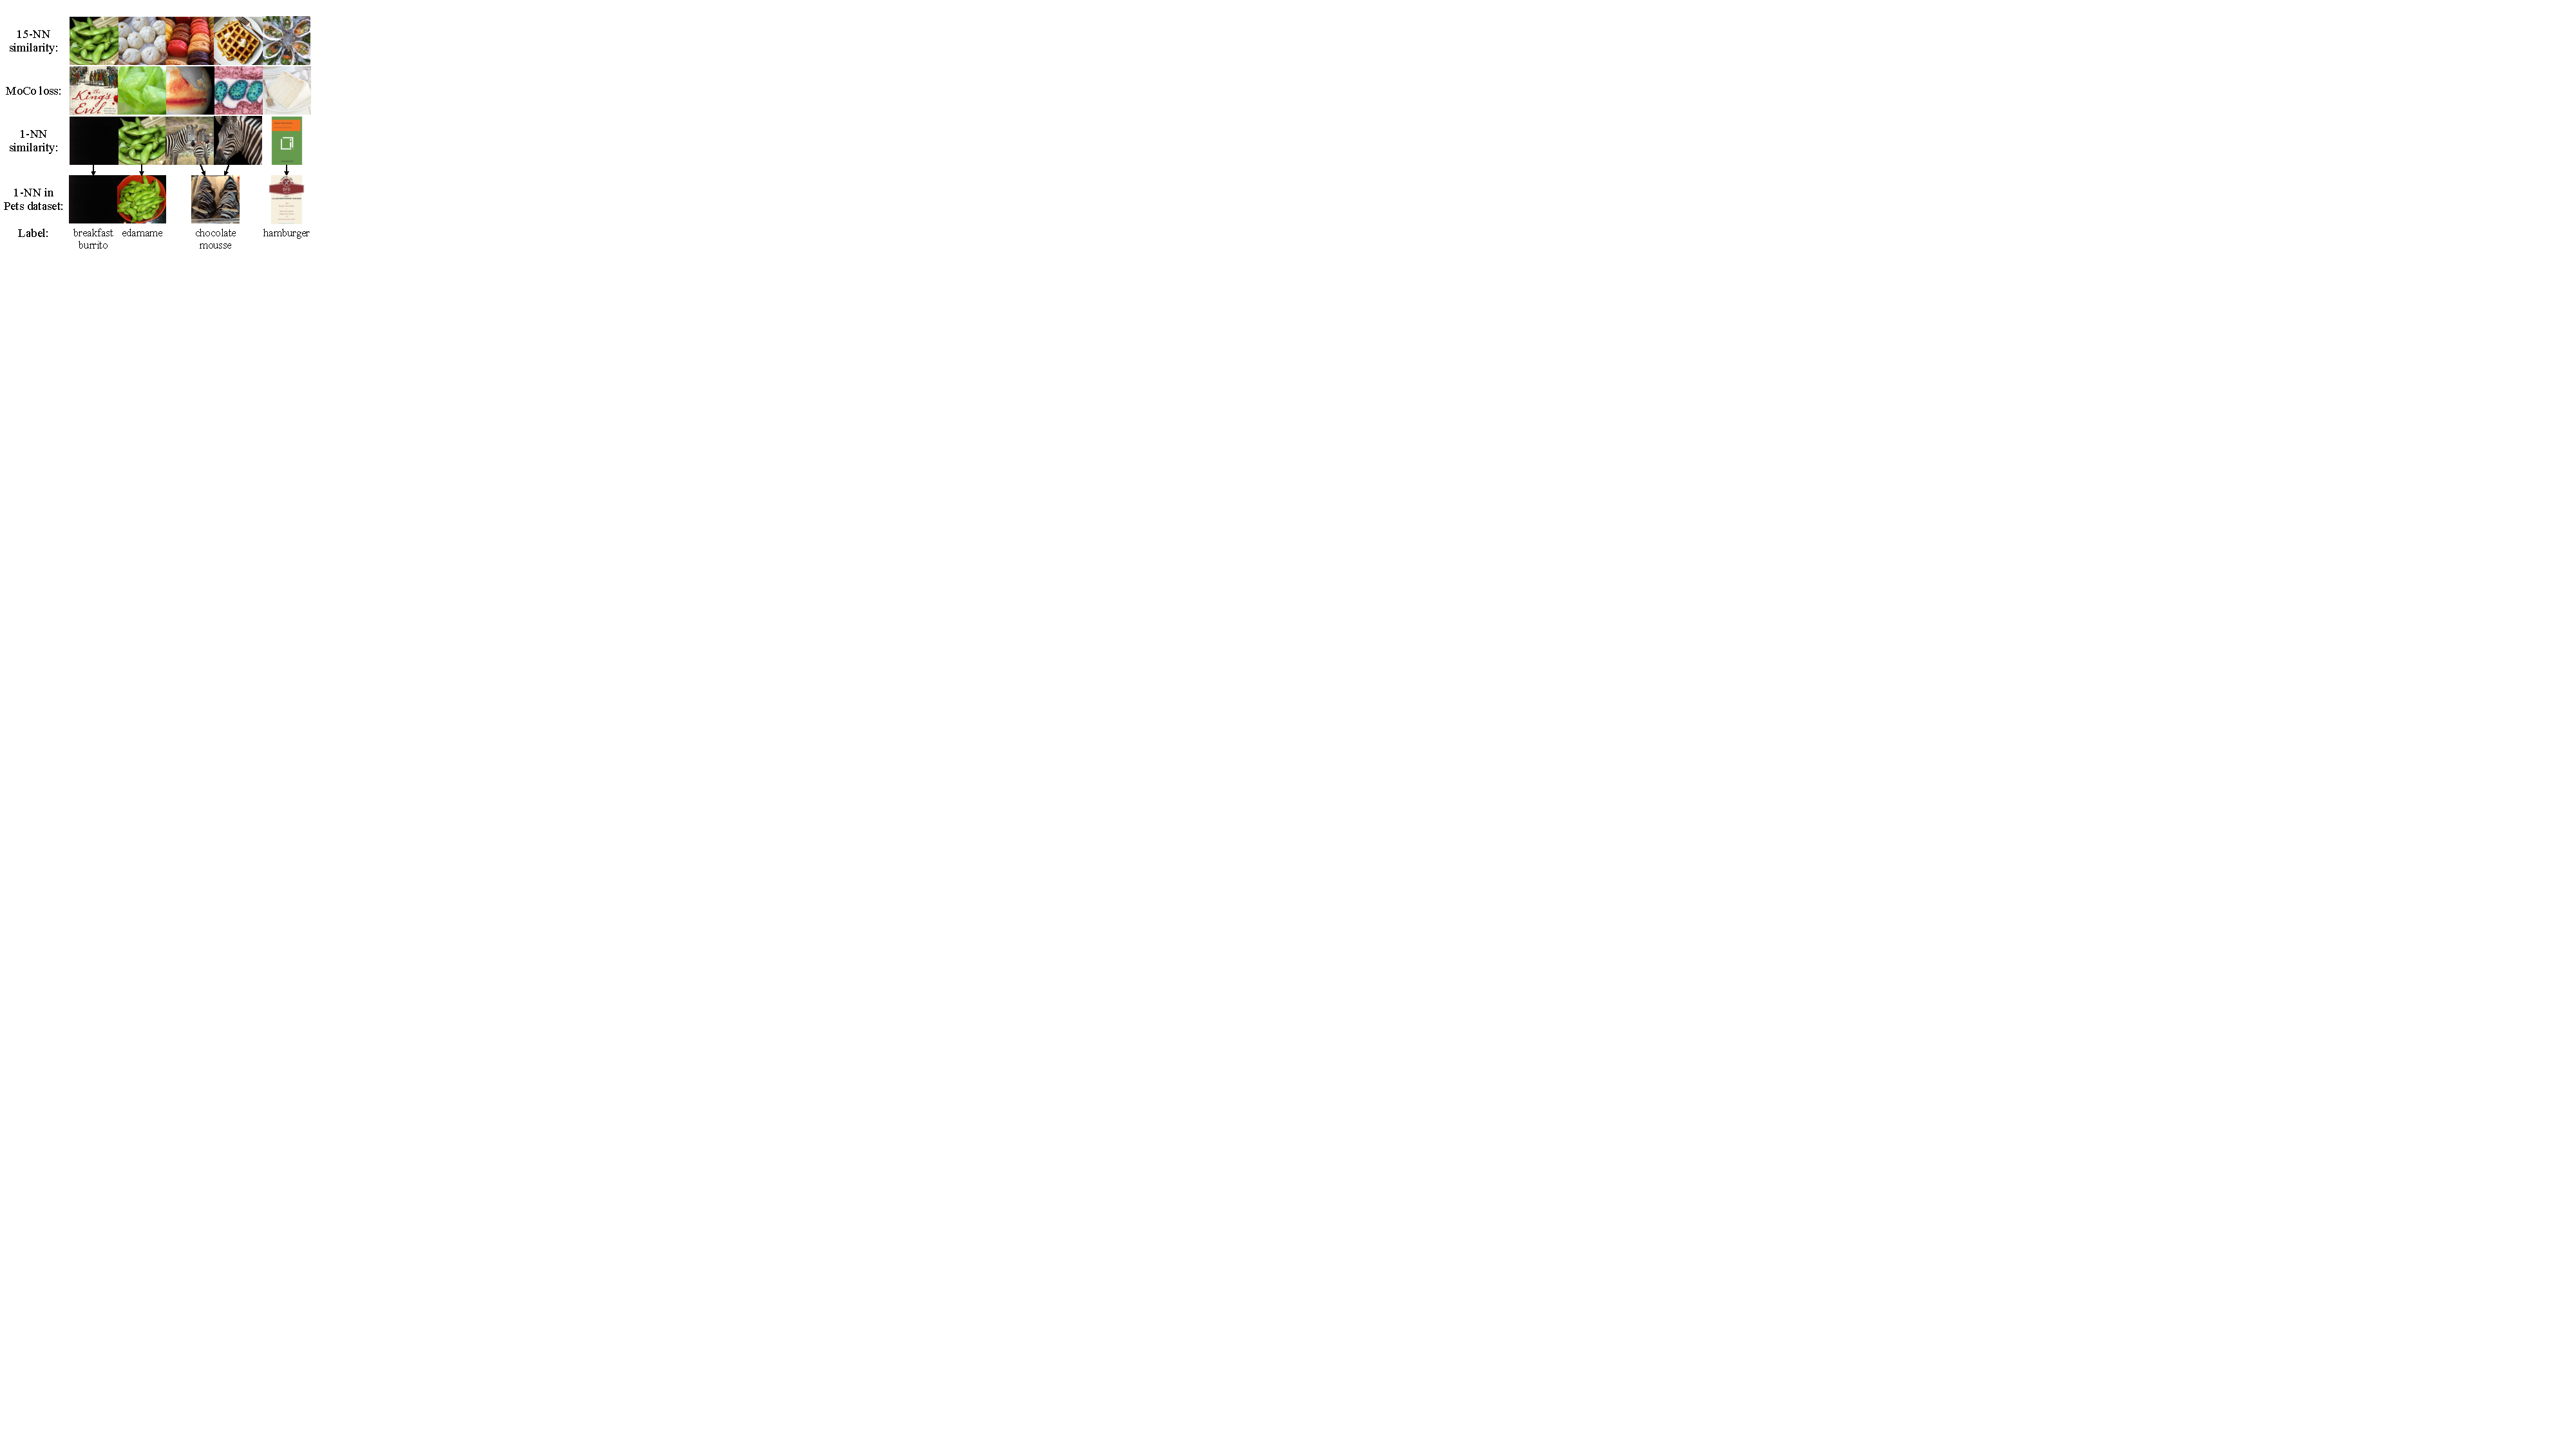
\includegraphics[width=0.5\linewidth]{figures/reward_ranking.pdf}
    % \vspace{-0.25in}
    \caption{\textbf{Top images preferred by different rewards.} We show the top 5 downloaded images ranked by 3 possible image rewards on the Food dataset. 15-NN (ours) prefers a variety of food images, whereas MoCo prefers noisy images out of the training distribution. 1-NN is thrown off by outliers in the Food dataset and thus prefers black images, text, and zebras.}
    \label{fig:reward_ranking}
    % \vspace{-0.06in}
\end{figure}

\subsection{Self-supervised Exploration Behavior on Other Datasets} 
\label{sec:progression_continued}
Just as \cref{fig:progression} in \cref{sec:exploration_behavior} showed how Internet Explorer progressively discovers useful data when targeting the Pets dataset, \cref{fig:birdsnap_progression}, \cref{fig:flowers_progression}, \cref{fig:food_progression}, and \cref{fig:voc_progression} show the progression of downloaded images when targeting Birdsnap, Flowers, Food, and VOC 2007 respectively. Note that this analysis is in the self-supervised setting, without any knowledge of the label set. 

\begin{figure*}
    \centering
    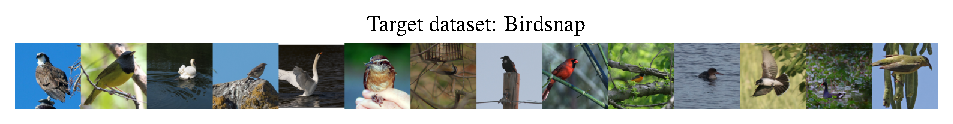
\includegraphics{figures/birdsnap_targets.pdf} \\
    \vspace{-0.8em}
    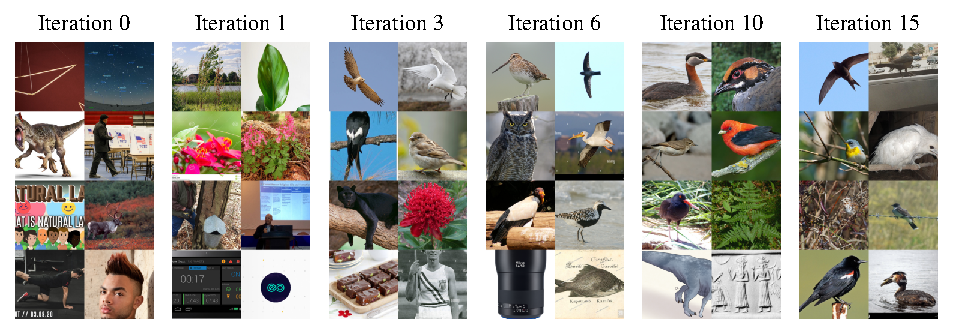
\includegraphics{figures/birdsnap-progression-1146-2col.pdf}
    \caption{\textbf{Progression of downloaded Birdsnap images.} This corresponds to Ours++ without using label set information. }
    \label{fig:birdsnap_progression}
\end{figure*}

\begin{figure*}
    \centering
    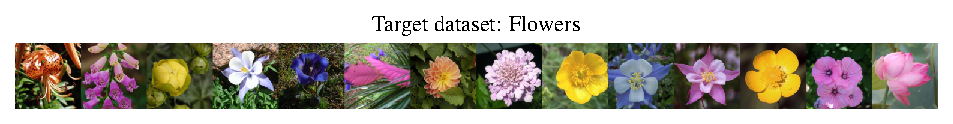
\includegraphics{figures/flowers_targets.pdf} \\
    \vspace{-0.8em}
    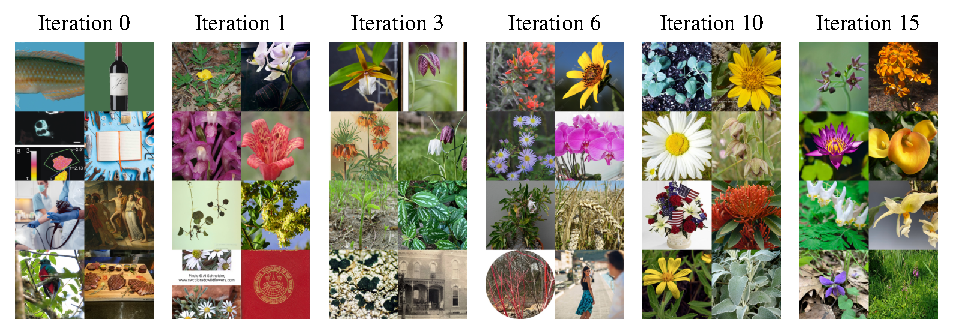
\includegraphics{figures/flowers-progression-1150-2col.pdf}
    \caption{\textbf{Progression of downloaded Flowers images.} This corresponds to Ours++ without using label set information. }
    \label{fig:flowers_progression}
\end{figure*}

\begin{figure*}
    \centering
    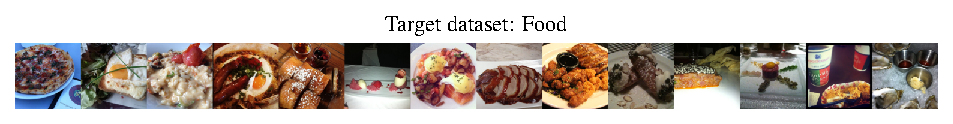
\includegraphics{figures/food_targets.pdf} \\
    \vspace{-0.8em}
    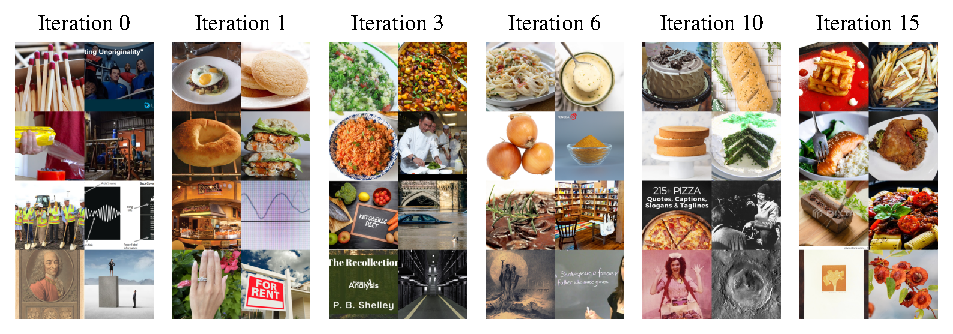
\includegraphics{figures/food-progression-1148-2col.pdf}
    \caption{\textbf{Progression of downloaded Food images.} This corresponds to Ours++ without using label set information. }
    \label{fig:food_progression}
\end{figure*}

\begin{figure*}
    \centering
    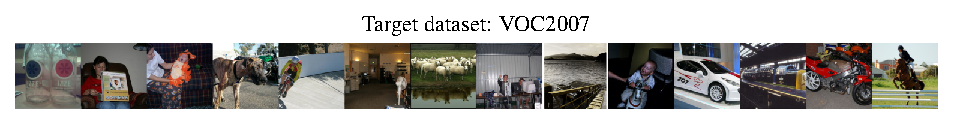
\includegraphics{figures/voc_targets.pdf} \\
    \vspace{-0.8em}
    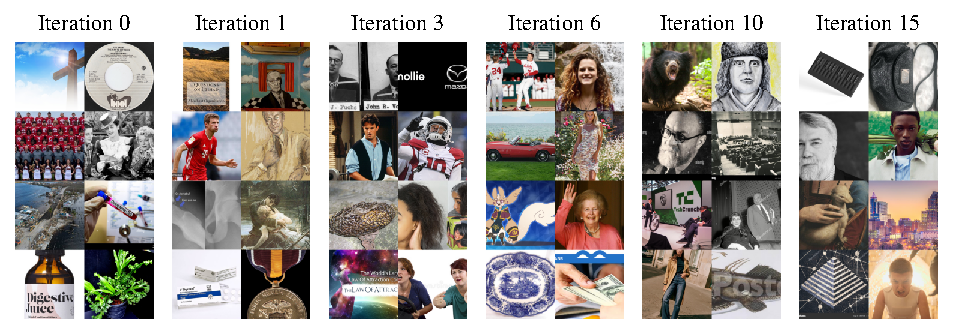
\includegraphics{figures/voc-progression-1156-2col.pdf}
    \caption{\textbf{Progression of downloaded VOC2007 images.} This corresponds to Ours++ without using label set information. }
    \label{fig:voc_progression}
\end{figure*}



%%% Local Variables:
%%% coding: utf-8
%%% mode: latex
%%% TeX-engine: xetex
%%% TeX-master: "../thesis"
%%% End:

\chapter{Conclusions and Future Directions}
\label{sec:conclusions}

In this thesis we have introduced new building blocks and
fundamental components for machine learning that enable
optimization-based domain knowledge to be injected
into the modeling pipeline.
We have presented the \emph{OptNet} architecture as a
foundation for convex optimization layers and the
\emph{input-convex neural network} architecture as a
foundation for deep convex energy-based learning.
We have shown how the OptNet approach can be applied to
differentiable model-predictive control and
top-$k$ learning.
To enable rapid prototyping in this space, we have shown
how \cvxpy can be turned into a differentiable layer.
Differentiable optimization provides an expressive set of
operations and have a promising set of future directions.
In the following we provide a brief outlook of how optimization-based
modeling benefits seven application areas,
and we highlight a few key references in this space.

\begin{enumerate}
\item \textbf{Game theory.}
  The game theory literature typically focuses on finding
  optimal strategies of playing games with known rules.
  While the rules of a lot of games are known explicitly,
  scenarios could come up where it's useful to learn the
  rules of a game and to have a ``game theory''
  equilibrium-finding layer.
  For example in reinforcement learning, an agent can have an
  arbitrary differentiable ``game theory'' layer that is able
  of representing complex tasks, state spaces, and
  problems as an equilibrium-finding problem in a game
  where the rules are automatically extracted.
  This is explored in
  \citet{ling2018game}.
\item \textbf{Stochastic optimization and end-to-end learning.}
  Typically probabilistic models are used in the context of
  larger systems. When these systems have an objective
  that is being optimized, it is usually ideal to incorporate
  the knowledge of this objective into the probabilistic modeling
  component.
  If the downstream systems involve solving
  stochastic optimization problems, as in power-systems,
  creating an end-to-end differentiable architecture is
  more difficult and can be done by using
  differentiable optimization as in \citet{donti2017task}.
  \newpage
\item \textbf{Reinforcement learning and control.}
  \begin{itemize}
  \item \textbf{Safety.} RL agents may be deployed in scenarios when
    the agent should avoid parts of the state space,
    \eg in safety-critical environments.
    Differentiable optimization layers can be used
    to help constrain the policy class so that these
    regions are avoided.
    This is explored in
    \citet{dalal2018safe,pham2018optlayer}.
  \item \textbf{Differentiable control and planning.}
    The differentiable MPC approach we presented in \cref{sec:empc}
    is just one step towards a significantly broader vision
    of integrating control and learning for doing imitation
    or policy learning.
  \item \textbf{Physics-based modeling.}
    When RL environments involve physical systems,
    it may be useful to have a physics-based modeling.
    This can be done with a differentiable
    physics engines as in \citet{de2018end}.
  \item \textbf{Inverse cost and reward learning.}
    Given observed trajectories in an imitation learning
    setup, modeling agents as controllers that are
    optimizing an objective is a powerful paradigm
    \citep{ng2000algorithms,finn2016guided}.
    Differentiable controllers
    are useful when trying to reconstruct an optimization
    problem that other agents are solving.
    This is done in the context of cost shaping in
    \citet{tamar2017learning}.
  \item \textbf{Multi-agent environments.}
    In multi-agent environments, other agents can be modeled
    as entities that are solving control optimization or
    other learning problems.
    This knowledge can be integrated into the learning
    procedure as in \citet{foerster2018learning}.
  \item \textbf{Control in high-dimensional state spaces.}
    Control in high-dimensional state spaces such as visual
    spaces is challenging and it is typically useful
    to extract a lower-dimensional latent space from
    the original feature space.
    This is typically done by either hand-engineering
    a feature extractor, or by learning an embedding
    with an unsupervised learning method as in
    \citet{watter2015embed,kurutach2018learning}.
    Viewing controllers as differentiable entities is
    reasonable for embedding states because the cost
    function of the controller can be parameterized to
    learn a cost associated with the latent representation.
  \end{itemize}
\item \textbf{Discrete, combinatorial, and submodular optimization.}
  The space of discrete, combinatorial, and mixed optimization problems
  captures an even more expressive set of operations than
  the continuous and convex optimization problems we have considered
  in this thesis.
  Similar optimization components can be made for some of these
  types of problems and is explored in
  \citet{djolonga2017differentiable,tschiatschek2018differentiable,mensch2018differentiable,niculae2018sparsemap,niculae2017regularized}.
  \newpage
\item \textbf{Meta-learning.}
  Some meta-learning formulations such as \citet{finn2017model}
  and \citet{ravi2016optimization}
  involve learning through an unrolled optimizer that
  typically solve an unconstrained, continuous, and
  non-convex optimization problem.
  In some cases, unrolling through a solver with
  many iterations may require inefficient amounts
  of compute or memory.
  Meta-learning methods can be improved by using
  differentiable closed-form solvers, as done in
  MetaOptNet \citep{lee2019meta} with a differentiable SVM layer
  and in \citet{bertinetto2018meta} with differentiable ridge
  and logistic regression.
\item \textbf{Optimization viewpoints of standard components.}
  A motivation behind this thesis work has been the optimization
  viewpoints of standard layers we discussed in \cref{sec:bg:existing}.
  Many other directions can be taken with the viewpoints, such
  as the proximal operator viewpoint in \citet{bibi2018deep}
  that interprets deep layers as stochastic solvers.
\item \textbf{Hyper-parameter and generalization optimization.}
  The learning procedure for many linear machine learning models
  can be interpreted as the solution to a convex
  optimization problem over the loss function.
  This convex learning process can therefore also be
  made differentiable and used for optimizing the hyper-parameters
  of these algorithms. This is done in
  \citet{barratt2018optimizing} to optimize the cross-validation
  risk of convex formulations, including logistic regression,
  SVMs, and elastic net regression;
  for least squares in \citet{barratt2019least};
  and SVMs in \citet{lee2019meta}.
\end{enumerate}

%%% Local Variables:
%%% coding: utf-8
%%% mode: latex
%%% TeX-engine: xetex
%%% TeX-master: "../thesis"
%%% End:

\chapter*{Bibliography}
\addcontentsline{toc}{chapter}{Bibliography}

\vspace{-25mm}
This bibliography contains \total{citenum} references.
\vspace{10mm}

\printbibliography[heading=none]

\end{document}

%%% Local Variables:
%%% coding: utf-8
%%% mode: latex
%%% TeX-engine: xetex
%%% End:
